\chapter{无人机视觉定位与堆体重建及体积测量测试与分析}
\label{cha:chap5}
\section{引言}
\label{sec:5.1}
本章将对以上章节提出的方法通过实验进行验证,主要包括无人机的自主定位和飞行精度测试,三维重建生成点云的实效性以及精度测试和面向堆体的体积精度测试。本章将对这三部分内容进行分模块处理,包括实验设计,方法测试,数据分析等,对方法表现进行定性分析,对实验数据进行定量比较。

对于无人机的自主定位和飞行精度测试,本章将对实际场景展开无人机的定位和飞行,结合第2章所提方法,利用场景中的二维码进行有尺度且基于真实世界坐标系下自主定位,并基于定位结果进行无人机的循迹飞行。在无人机飞行的过程中,实时记录下无人机的飞行状态,和二维码地图的数据,对精度进行定量分析。

对于三维重建生成点云的实效性以及精度测试,本章将对比第3章所提出的稀疏点云重建所采用的图像匹配模式,定性比较各匹配模式之间的实效性,并结合SLAM将运行后的keyFrame DataBase以及先验位姿提供给离线三维重建系统,定性比较三维重建后点云的精度差异。

对于面向堆体的体积测量精度测试,本文选用沙堆作为研究对象,利用其易获取真值且能够任意改变形状的特点,代替其他堆体进行试验。结合第4章的方法,测试堆体三维点云和实际堆体之间的尺度估计值,堆体点云的水平面方程,以及利用纯视觉方法测试堆体体积的稳定性和精确度。
\section{无人机视觉定位系统测试与分析}
\label{sec:5.2}
\subsection{无人机视觉定位系统实验步骤设计}
\label{sec:5.2.1}
在第2章,本文提出了一种结合二维码的SLAM视觉定位系统,利用该系统可以估计出带有真实尺度的相机位姿,以及能够得到真实世界坐标系下的相机位姿。本次实验主要利用上述方法在不利用GPS信号的环境下,结合二维码视觉标签进行无人机定位,通过获得到的位置信息进行下一步的飞行控制。本次实验的准备过程主要分为三个步骤,布置场景,生成地图,无人机循迹飞行。

首先是场景布置,选择在空旷场地中,布置二维码视觉标签,保证每个二维码的尺度大小完全一致,且二维码之间尽可能等间距布置,场景中的二维码ID完全独立不同,设计图和实际布置图分别如图~\ref{fig:5Test_scene_imagine}和图~\ref{fig:5Test_scene_reality}所示。在本次实验中,所原选择的二维码实际大小为0.73m,相邻二维码之间的距离为4m,整个实验区域面积为400$m^2$(20m*20m)。
\begin{figure}[H]
  \centering%
  \subcaptionbox{实验场景设计示意图\label{fig:5Test_scene_imagine}}{%    
    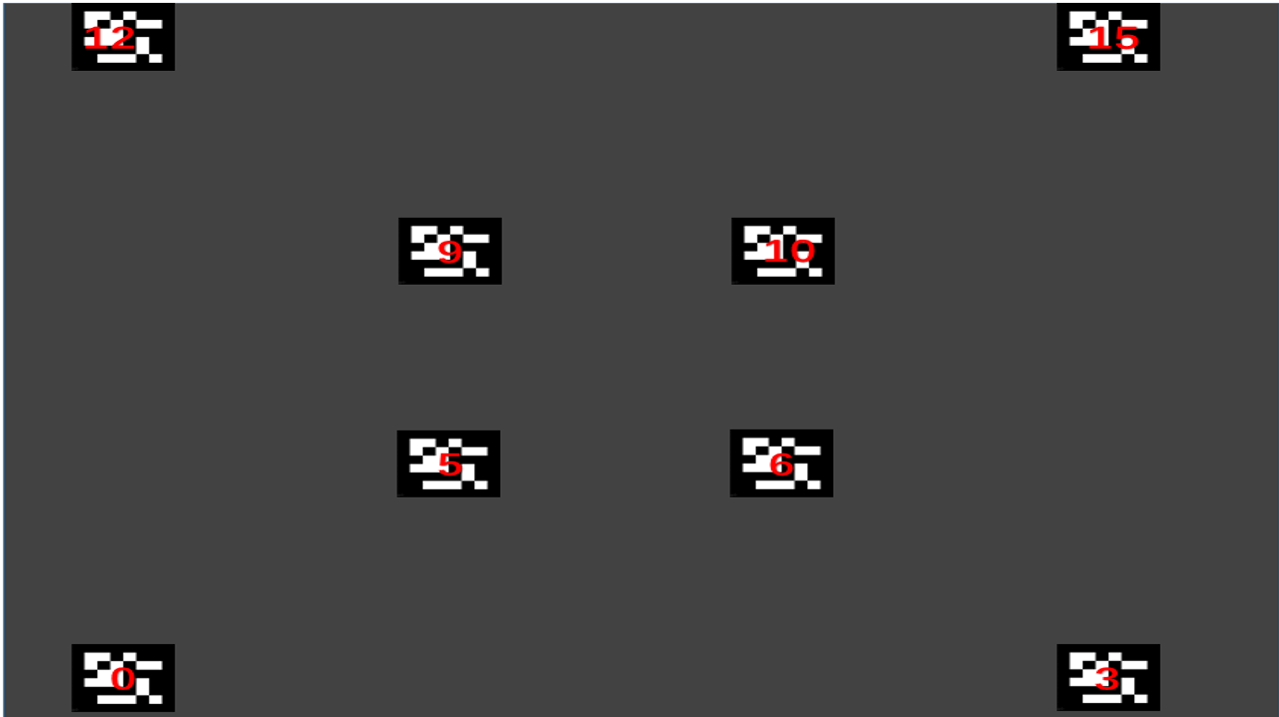
\includegraphics[height=4.5cm,width=4.5cm]{5Test_scene_imagine.png}}\hspace{4em}%
  \subcaptionbox{实验场景真实布置图\label{fig:5Test_scene_reality}}{%    
    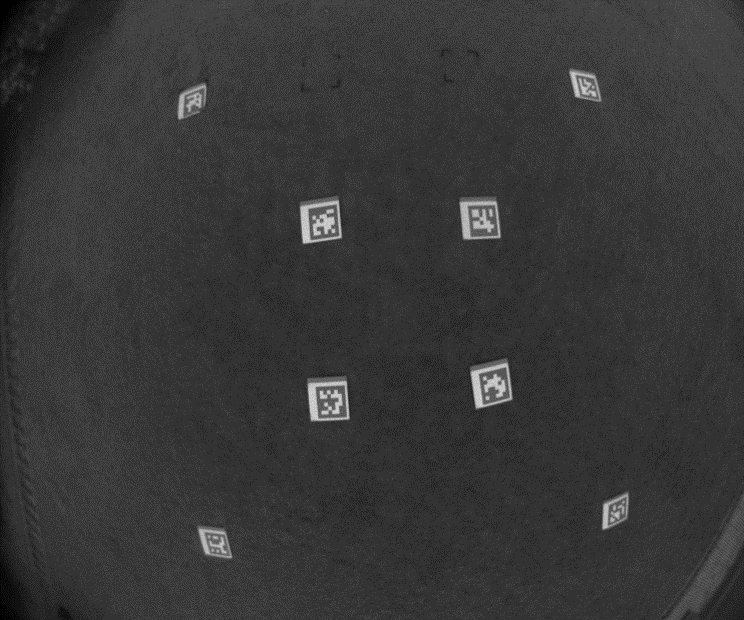
\includegraphics[height=4.5cm,width=4.5cm]{5Test_scene_reality.png}}
  \caption{实验场景示意图}
  \label{fig:scene}
\end{figure}

在布置好场景后,需要根据实际场景生成地图信息。当无人机首次在无先验地图的环境下飞行时,为了保证后续飞行精度,可以先飞行一次建立场景的先验地图,在无人机的飞行过程中,其飞行区域需要尽可能覆盖所有场景以确保生成完整的地图,根据实际场景生成的地图如图~\ref{fig:5Test_map_generator}所示,其中正方形框代表二维码,蓝色相机表示代表视觉定位产生的关键帧,点代表地图中的特征点。
\begin{figure}[H] % use float package if you want it here
  \centering
  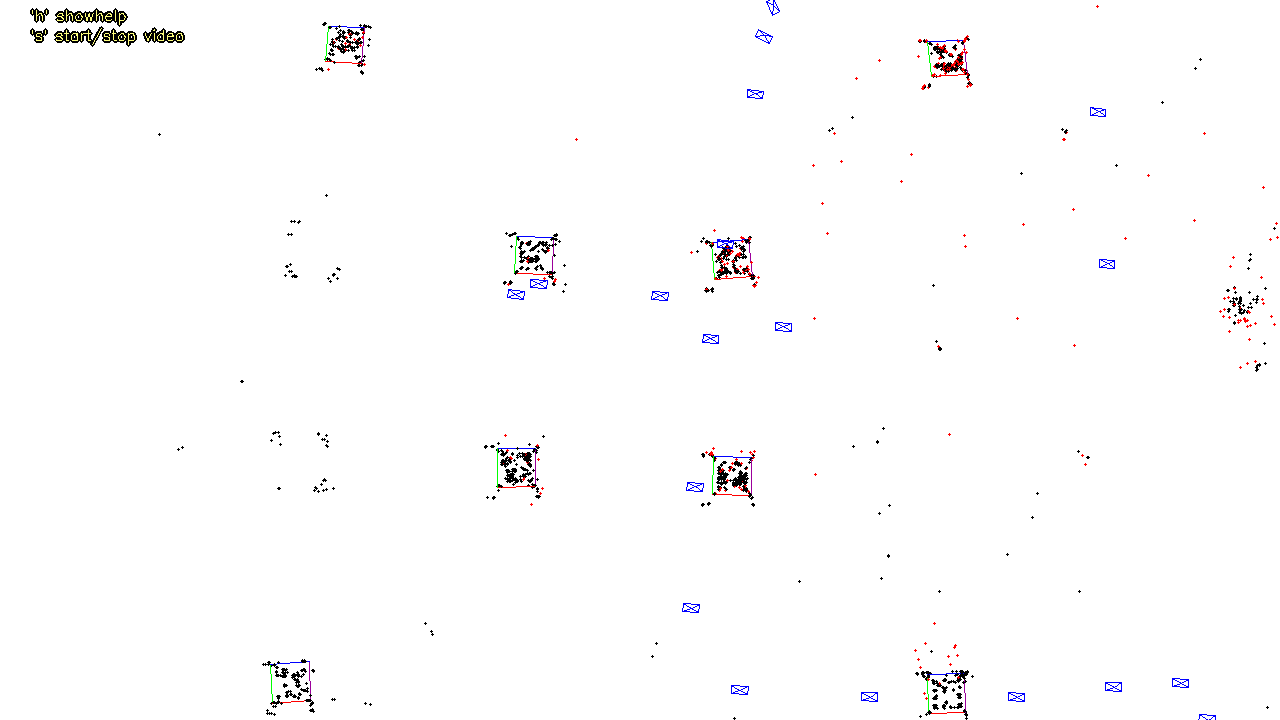
\includegraphics[height=5cm]{5Test_map_generator.png}
  \caption{视觉算法生成地图}
  \label{fig:5Test_map_generator}
\end{figure}
当获取到完整的地图信息地图后,可以让无人机按照认为规定的轨迹进行自动循迹飞行,首先设计如下图~\ref{fig:5Test_flight_route}所示的轨迹图,起飞点为ID=0的二维码处,红色箭头代表无人机的飞行轨迹,对于无人机的飞控过程,按照设定循迹点的方案来实现,在整个轨迹中给定多个循迹点坐标,使得无人机按照设定的坐标顺序进行飞行即可。
\begin{figure}[H] % use float package if you want it here
  \centering
  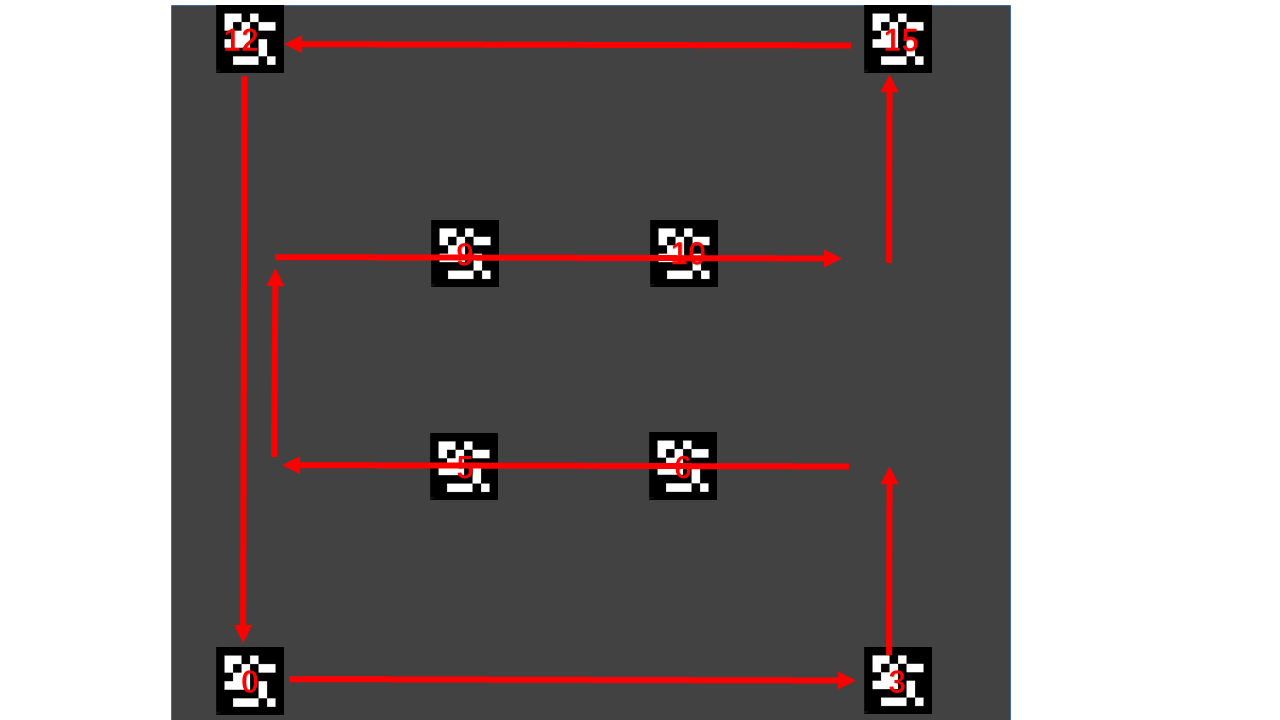
\includegraphics[height=5cm]{5Test_flight_route.png}
  \caption{无人机自主飞行轨迹设计图}
  \label{fig:5Test_flight_route}
\end{figure}
\subsection{视觉定位系统实验结果分析}
\label{sec:5.2.2}
按照上述实验流程让无人机进行自主飞行,可以直接获得视觉算法生成的地图以及无人机在飞行的过程中生成的三维坐标,根据这些数据可以对视觉算法关于无人机自主定位的效果进行定量的分析,本文主要从生成地图的精度,无人机三维坐标的精度以及轨迹精度三个方面进行定量分析。

首先对于地图精度,根据图~\ref{fig:5Test_scene_reality}生成的地图,通过对地图的解析,可以获取每一个二维码的三维位置坐标,如表~\ref{tab:chap1:marker_pose}所示。
\begin{table}[h]
  \centering
  \caption{二维码标志位置实际测量值}
  \label{tab:chap1:marker_pose}
  \begin{tabular}{C{3.6cm}L{2.4cm}L{2.4cm}L{2.4cm}}
  \toprule
  \textbf{序号} & \textbf{X} & \textbf{Y} & \textbf{Z} \\
  \midrule
  0      & -2.63   & 	1.32 & 7 .86            \\
  3      & -14.69  & 	3.88 & 7.80            \\
  5      & -6.05 	 &  6.34 & 7.45           \\
  6      & -9.83 	 &  -9.83 & 7.45           \\
  9      & -5.13 	 &  10.44 & 7.30           \\
  10     & -9.17   &	11.22 &	7.24        \\
  12     & -0.33 	 &  13.56 & 7.34 	             \\
  15     & -12.25  & 	16.15 &	7.27            \\
  \bottomrule
  \end{tabular}
\end{table}
针对地图的精度,可以提出以下两个判断指标:

1. 任意两个二维码之间距离的测量值和理论值的误差比较;

2. 所有二维码是否在同一个坐标平面。

针对指标1,计算得到表~\ref{tab:chap1:marker_map_error},经过计算得到地图中二维码的平均误差精度为3.1$\%$。
\begin{table}[h]
    \centering
    \caption{二维码位置误差}
    \label{tab:chap1:marker_map_error}
    \begin{tabular}{C{1.6cm}C{1.6cm}C{2.4cm}C{2.4cm}C{3.2cm}}
    \toprule
    \textbf{ID1} & \textbf{ID2} & \textbf{实际值} & \textbf{理论值} & \textbf{误差率} \\
    \midrule
    0&	3&	12.33&	12&	2.75 $\%$\\
    0&	5&	6.07&	5.65&	7.43$\%$\\
    0&	6&	9.26&	8.94&	3.58$\%$\\
    0&	9&	9.46&	8.94&	5.82$\%$\\
    0&	10&	11.86&11.31&	4.86$\%$\\
    0&	12&	12.45&	12&	3.75$\%$\\
    0&  15&	17.67&	16.97&	4.12$\%$\\
    3&	5&	8.99&	8.94&	0.56$\%$\\
    3&	6&	5.85&	5.65&	3.54$\%$\\
    3&	9&	11.6&	11.31&	2.56$\%$\\
    3&	10&	9.18&	8.94&	2.68$\%$\\
    3&	12&	17.32&	16.97&	2.06$\%$\\
    3&	15&	12.51&	12&	4.25$\%$\\
    5&	6&	3.87&	4&	3.25$\%$\\
    5&	9&	4.21&	4&	5.25$\%$\\
    5&	10&	5.79&	5.65&	2.48$\%$\\
    5&	12&	9.21&	8.94&	3.02$\%$\\
    5&	15&	11.61&	11.31&	2.65$\%$\\
    6&	9&	5.75&	5.65&	1.77$\%$\\
    6&	10&	4.13&	4&	3.25$\%$\\
    6&	12&	11.47&	11.31&	1.41$\%$\\
    6&	15&	9.33&	8.94&	4.36$\%$\\
    9&	10&	4.11&	4&	2.75$\%$\\
    9&	12&	5.72&	5.65&	1.24$\%$\\
    9&	15&	9.12&	8.94&	2.01$\%$\\
    10&	12&	9.15&	8.94&	2.35$\%$\\
    10&	15&	5.81&	5.65&	2.83$\%$\\
    12&	15&	12.2&	12&	1.67$\%$\\  
    \bottomrule
    \end{tabular}
\end{table}

针对指标2,绘制出每个二维码在同一个坐标平面的误差情况,如图~\ref{fig:5Test_marker_map_error_Z}所示,平均误差为0.18m,可以认定所有二维码基本都在同一水平面内。
\begin{figure}[H] % use float package if you want it here
  \centering
  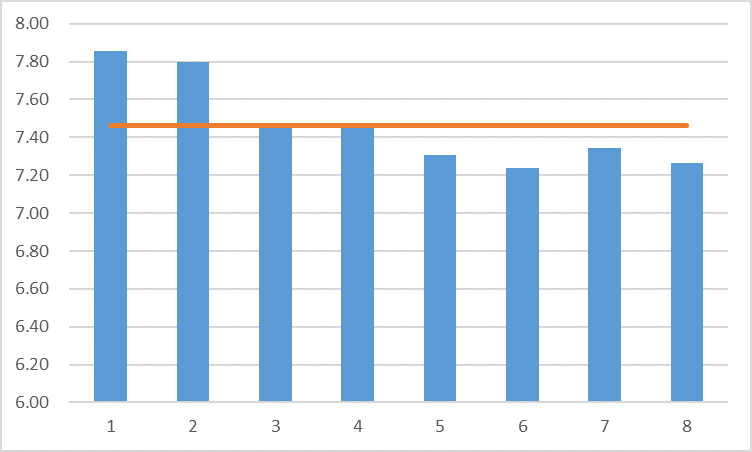
\includegraphics[height=6cm]{5Test_marker_map_error_Z.png}
  \caption{二维码Z方向数据}
  \label{fig:5Test_marker_map_error_Z}
\end{figure}
其次对于无人机三维坐标的精度,以无人机自带GPS测定出的坐标为真值,和视觉算法计算出来的位置信息进行对比,选择无人机800帧的数据,在X、Y、Z三个方向得到的结果分别如图~\ref{fig:5Test_pose_xyz}所示,其中蓝色连线为视觉算法检测出的坐标值,红色连线无人机GPS检测出的真实值。
\begin{figure}[h]
  \centering
    \subcaptionbox{X方向GPS和视觉算法对比图}{\label{fig:chap1:pose_x}
    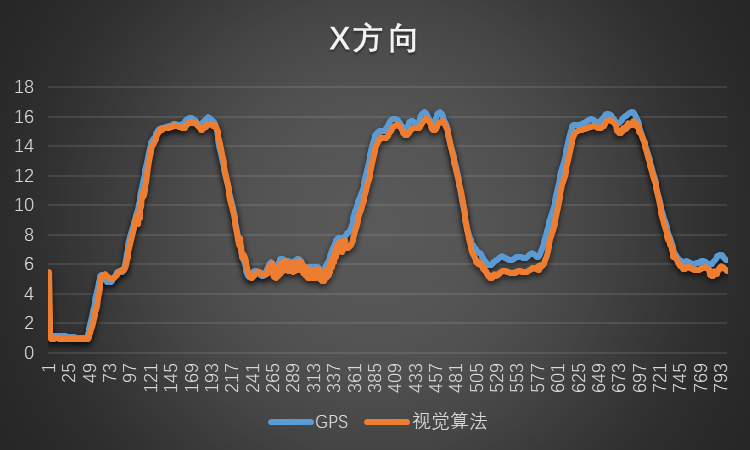
\includegraphics[width=5.5cm]{pose_x.png}\hskip2cm}
    \subcaptionbox{Y方向GPS和视觉算法对比图}{\label{fig:chap1:pose_y}
    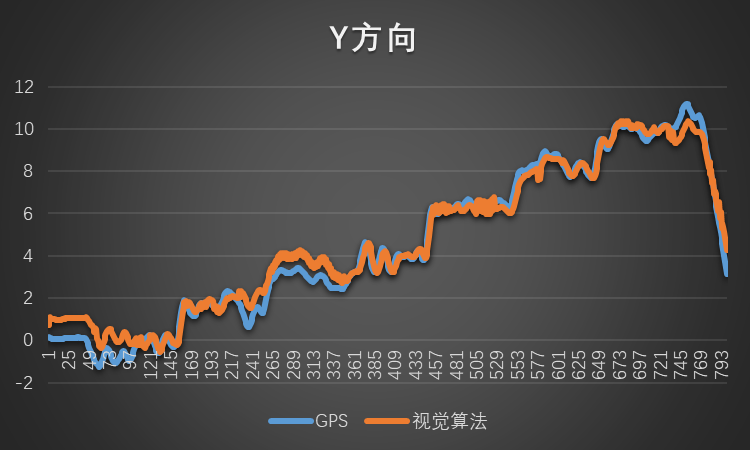
\includegraphics[width=5.5cm]{pose_y.png}}
  \vskip0.5cm
    \subcaptionbox{Z方向GPS和视觉算法对比图}{\label{fig:chap1:pose_z}
    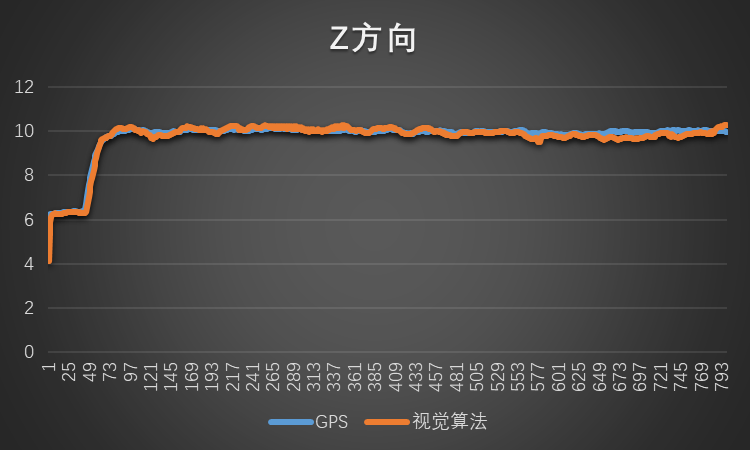
\includegraphics[width=5.5cm]{pose_z.png}}
  \caption{各方向GPS和视觉算法对比图}\label{fig:5Test_pose_xyz}
\end{figure}
随后,计算真值和测量值之间的误差,在X、Y、Z方向分别得到结果如图~\ref{fig:5Test_pose_error_xyz}所示,对于X、Y、Z三个方向分别可以得到距离误差为0.22m、0.37m、0.107m。
\begin{figure}[H]
    \centering
      \subcaptionbox{X方向GPS和视觉算法对比图}{\label{fig:chap1:pose_error_x}
      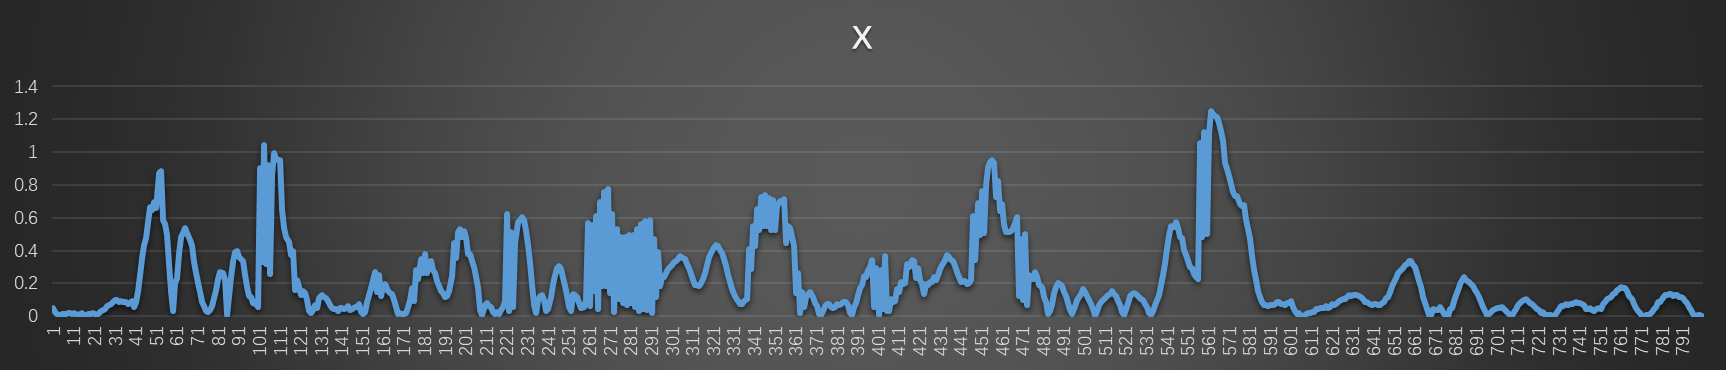
\includegraphics[width=10cm]{pose_error_x.png}}
    \vskip0.35cm
      \subcaptionbox{Z方向GPS和视觉算法对比图}{\label{fig:chap1:pose_error_y}
      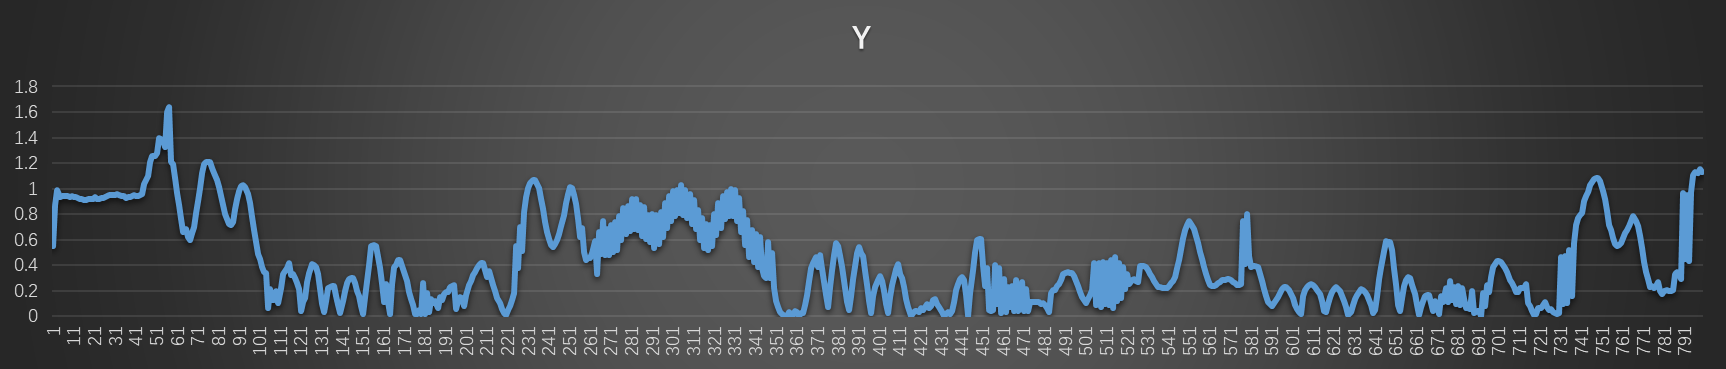
\includegraphics[width=10cm]{pose_error_y.png}}
    \vskip0.35cm
      \subcaptionbox{Z方向GPS和视觉算法对比图}{\label{fig:chap1:pose_error_z}
      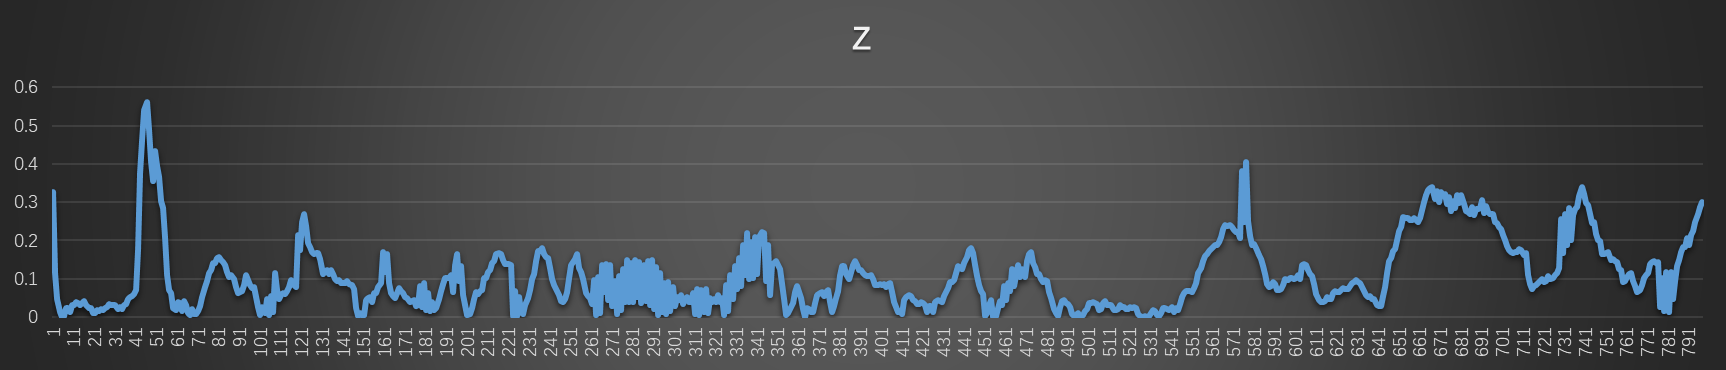
\includegraphics[width=10cm]{pose_error_z.png}}
    \caption{各方向GPS和视觉算法误差对比图}\label{fig:5Test_pose_error_xyz}
\end{figure}
最后,对无人机的轨迹精度进行对比。无人机在自主飞行过程中能够产生实时的相对于真实世界坐标系的定位信息,将其与GPS生成的定位信息进行对比,如图~\ref{fig:5Test_pose_map}所示。
\begin{figure}[H] % use float package if you want it here
  \centering
  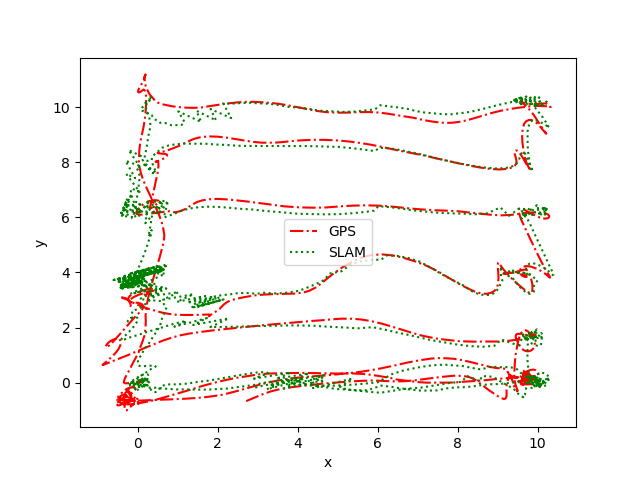
\includegraphics[height=8cm]{5Test_pose_map.png}
  \caption{无人机轨迹对比示意图}
  \label{fig:5Test_pose_map}
\end{figure}
对于无人机的直飞路线,误差较小,GPS和视觉算法测算出的轨迹基本吻合,但在转弯方向改变的区间,两者之间的相对误差则较大,考虑其原因为在转弯处所设计的循迹点相对比较稠密,导致在该区域内无人机需要改变的方向更大,视觉算法在测算时由于方法振动的缘故产生较大的误差。
\section{三维重建系统测试与分析}
\label{sec:5.3}
在本文~\ref{sec:3.2.3}节中,提出了三维重建存在的一些问题,包括对场景进行三维重建时,匹配耗时严重和点云准确性较低,甚至无法重建出三维点云,
本实验将结合~\ref{sec:3.3}节提出的方法对三维重建进行改进。
\subsection{匹配实效性测试}
通过~\ref{sec:3.3.2}节对输入图像匹配模式的分析,本实验共选择150张图像(图片选择过少的话,各匹配模式之间的耗时差异会过小)作为输入图片,每张图像的大小为960*544。各匹配模式包括完全匹配,序列匹配,空间匹配,传递匹配和自定义匹配,对于空间匹配,在对室内堆体三维重建时,难以获取准确的空间位置信息,本实验将排除该匹配方式的对比

其中自定义匹配以实时运行的SLAM匹配信息作为匹配结果。SLAM处理代码如~\ref{code:SLAM_process}下:
\begin{lstlisting}[
  language=C++,
  numbers=left,                
  numberstyle=\footnotesize,
  frame=single,     
  basicstyle=\small\tt,    
  escapeinside = '',
  caption={SLAM处理数据集~C++~实现},
  label={code:SLAM_process}]
'//SLAM处理数据集'

if (mpCurrentKeyFrame->mnId > 4)
  {

   std::vector<KeyFrame*> cos = 
    mpCurrentKeyFrame->GetBestCovisibilityKeyFrames(covisibleNum);
   cv::Mat rotation = mpCurrentKeyFrame->GetRotation();
   cv::Mat translation = mpCurrentKeyFrame->GetTranslation();

   Eigen::Matrix3d r2 = Converter::toMatrix3d(rotation);
   Eigen::Quaterniond q2(r2);

   fs1 << mpCurrentKeyFrame->mnFrameId << ",";
   for (int k = 0; k < cos.size(); k++)
   {
    fs1 << cos[k]->mnFrameId << ",";
   }

   fs1 << "|" << 
   q2.w() <<","<< q2.x() <<","<< q2.y() <<","<< q2.z() <<","
   << translation.at<float>(0) <<","
   << translation.at<float>(1) <<","
   << translation.at<float>(2) 
   << std::endl;
  }
\end{lstlisting}
对任意一帧图像,在SLAM处理后只处理并保存关联关键帧大于4帧的图像,依次获取与该帧匹配度最高的4帧和该帧所对应的位姿(R,t),结果如表~\ref{tab:SLAM_result}所示。
\begin{table}[h]
  \centering
  \caption{SLAM处理结果}
  \label{tab:SLAM_result}
  \begin{tabular}{C{1.2cm}C{4.0cm}C{8.6cm}}
  \toprule
  \textbf{当前帧} & \textbf{匹配帧集合} &\textbf{位姿}  \\
  \midrule
  4&[5 3 2 1 ]&[R:0.989 -0.008 -0.137 0.053 t:-0.00 0.017 -0.033]\\
  3&[4 5 2 1 ]&[R:0.989 -0.031 -0.163 0.056 t:-0.001 0.015 -0.030]\\
  6&[5 7 4 8 ]&[R:0.987 -0.019 -0.131 0.090 t:-0.018 0.016 -0.064]\\
  2&[3 4 5 1 ]&[R:0.981 -0.018 -0.184 0.057 t:0.000 0.015 -0.025]\\
  8&[9 7 10 6 ]&[R:0.989 -0.039 -0.111 0.079 t:-0.034 0.014 -0.104]\\
  $\dots$   &   $\dots$ &   $\dots$\\
  $\dots$   &   $\dots$ &   $\dots$\\
  $\dots$   &   $\dots$ &   $\dots$\\
  $\dots$   &   $\dots$ &   $\dots$\\
  145&[147 146 148 149 ]&[R:0.978 -0.118 -0.148 0.083 t:0.026 0.030 0.117]\\
  149&[148 147 146 145 ]&[R:0.983 -0.109 -0.114 0.083 t:0.0123 0.020 0.033]\\
  146&[147 148 145 149 ]&[R:0.972 -0.148 -0.168 0.067 t:0.017 0.0334 0.099]\\
  151&[4 5 152 3 ]&[R:0.989 -0.096 -0.099 0.047 t:0.001 0.010 -0.057]\\
  154&[12 13 11 10 ]&[R:0.992 -0.080 -0.085 0.021 t:-0.030 0.004 -0.204]\\
  \bottomrule
  \end{tabular}
\end{table}
各个匹配模式之间的耗时情况和匹配准确度如表~\ref{tab:match_compare}所示。
\begin{table}[h]
  \centering
  \caption{各匹配模式耗时与精度情况对比表}
  \label{tab:match_compare}
  \begin{tabular}{C{3.6cm}C{2.4cm}L{2.4cm}L{2.4cm}C{3.6cm}}
  \toprule
  \textbf{匹配模式} & \textbf{耗时(/s)} &\textbf{匹配精度}  \\
  \midrule
  完全匹配  &504& 精度较高\\
  序列匹配  &94&精度较高\\
  传递匹配  &7 &精度较差\\
  自定义匹配  &实时得到结果 &精度高\\
  \bottomrule
  \end{tabular}
\end{table}
由表可以分析得到,以SLAM实时运行的匹配结果作为三维重建的匹配输入,一方面可以节省下匹配所耗费的时间,另外SLAM通过对时序图像的分析,可以得到更加准确的匹配信息。
\subsection{点云精度测试}
在面对部分重复度高,表面问题贫瘠的场景中,三维重建往往难以生成有效的点云,按照第3.3.2节提出的方法可以以SLAM生成的keyFrame Database等信息作为先验知识来改善三维重建的结果。本实验考虑到地下车库场景重复度高,且存在反光现象,选择了地下车库作为实验场景,按照环形有闭环的路径采集了一系列图像,部分图像如~\ref{fig:5Test_3D_garage}所示。
\begin{figure}[H] % use float package if you want it here
  \centering
  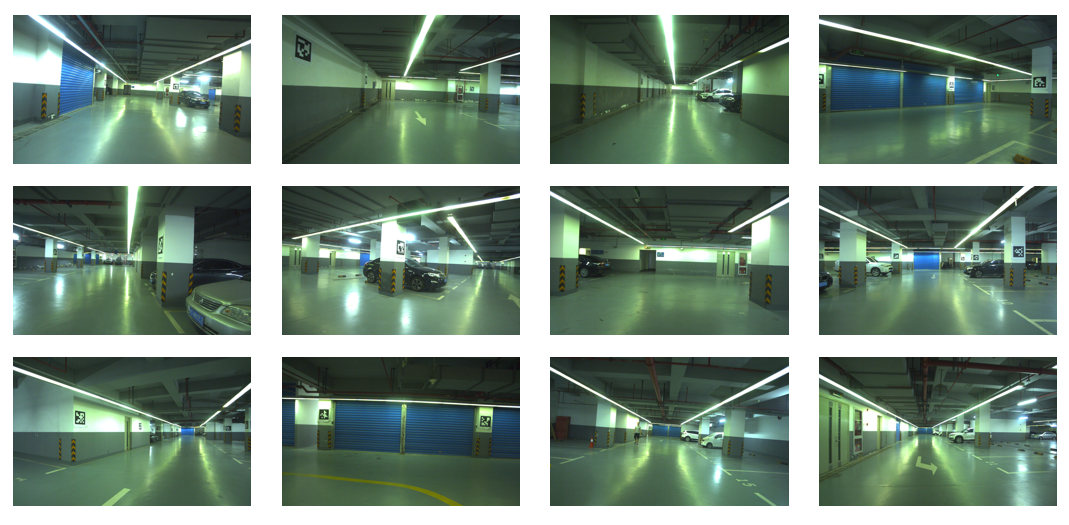
\includegraphics[height=5cm,width=9.7cm]{5Test_3D_garage.png}
  \caption{地下车库环形图像}
  \label{fig:5Test_3D_garage}
  \end{figure}
分别以传统方法和改进后的方法对其进行三维重建,结果分别如图~\ref{fig:test_3D_badresult}和~\ref{fig:test_3D_goodresult}所示。
\begin{figure}[h]
  \centering
    \subcaptionbox{结合SLAM三维重建\label{fig:test_3D_badresult}}{
    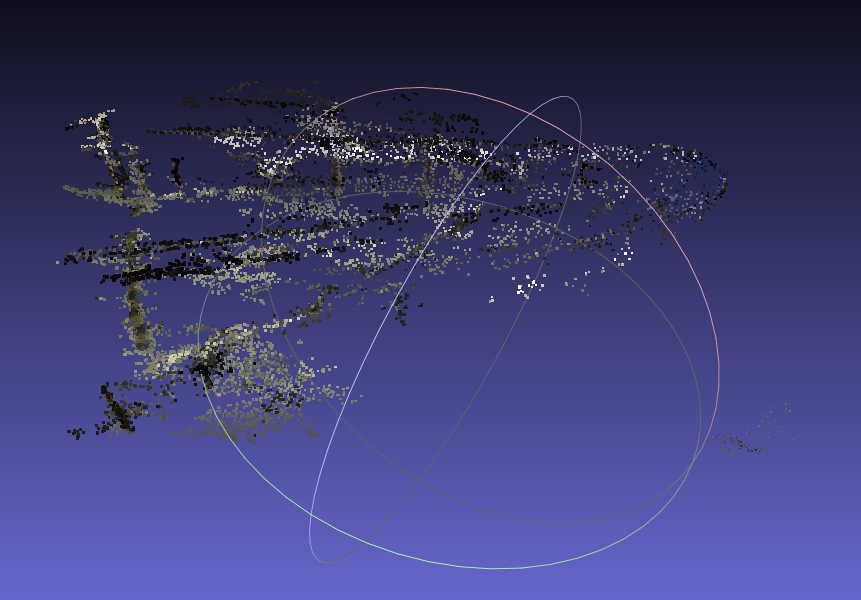
\includegraphics[height=5cm,width=9.7cm]{test_3D_badresult.png}}
  \vskip0.5cm
    \subcaptionbox{直接三维重建\label{fig:test_3D_goodresult}}{
    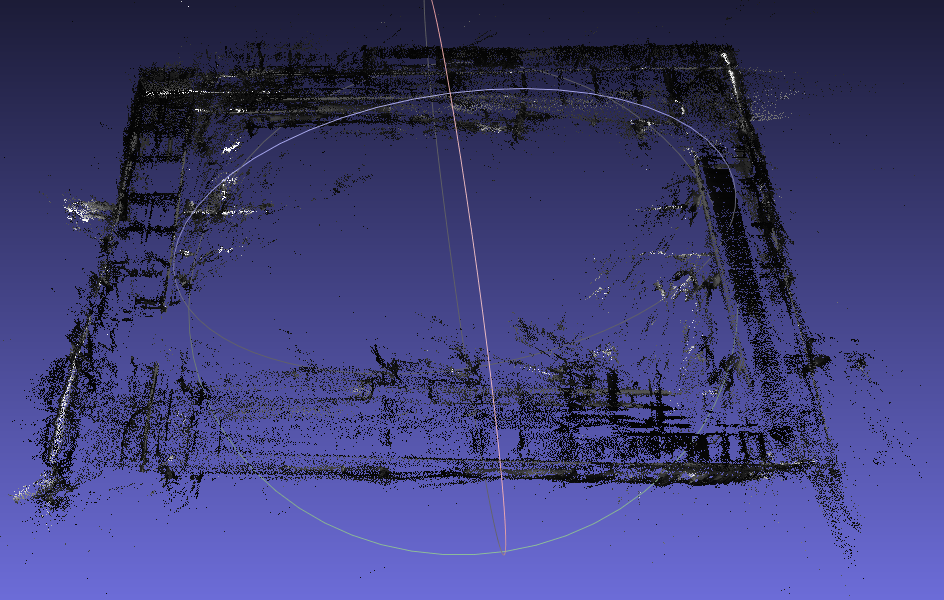
\includegraphics[height=5cm,width=9.7cm]{test_3D_goodresult.png}}
  \caption{地下车库三维重建对比图}\label{fig:test_3D}
\end{figure}
对于普通三维重建方法而言,地下车库场景重建场景点云难度较大,因为场景中的场景重复度高,匹配精度较低,且反光场景的加入又会导致相机的位姿估计出现偏差,三维重建无法生成有效的点云结果。因此需要结合SLAM的结果来作为三维重建的先验知识,提供更多丰富的匹配约束以及更加精准的相机位姿,可以重建出较好的结果。
\section{堆体体积测量系统测试与分析}
\label{sec:5.4}
在第4章,本文提出了一种基于纯视觉方法来测量堆体体积的方法,基于对实验场景进行的三维重建结果,整个实验步骤主要包括以下四个方面:

1. 解析水平面方程

2. 估计场景实际尺度

3. 点云提纯

4. 计算三维点云的体积。

在测量堆体场景体积之前,需要收集该场景的连续视频帧以获取其三维重建的结果,考虑到稠密点云的点集数量过大,在遍历和查询时都会比较耗时,且稀疏点云也包含了每个特征点的坐标信息和相机的位姿信息,后续在解析水平面方程和估计场景实际尺度时选择稀疏点云作为分析对象。

\subsection{解析水平面方程}
\label{sec:5.4.1}
1. 场景布置:在待测堆体场景中需要布置多个不同的二维码,一方面提高场景三维重建的稳定性和准确性,另外进一步为后续水平面方程的解析提供数据。在布置场景时,需要注意两个问题:1)布置的二维码的所有下边沿都位于同一条直线上;2)应该尽可能将所有Aruco的二维码的下边沿都与待求水平面贴合,以保证水平面方程求解的准确性,若无法实现水平面的贴合要求,则需要进一步保证所有下边沿都位于同一水平面上,那么对计算得到的水平面进行空间变换即可得到真实水平面方程。

2. 数据收集:可以通过单目相机对堆体场景进行连续采集,在采集视频的过程中需要保证大部分图像帧中都能够采集到完整的二维码,所有的采集结果如图~\ref{fig:5Test_inputCamera}所示。
\begin{figure}[H] % use float package if you want it here
  \centering
  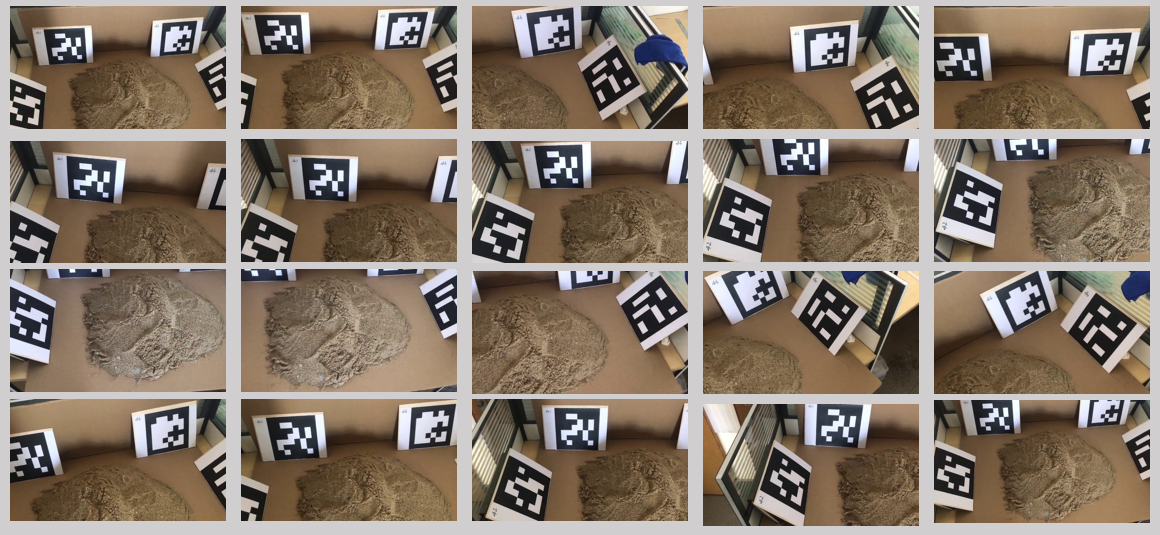
\includegraphics[height=5.5cm]{5Test_inputCamera.png}
  \caption{堆体场景图像序列}
  \label{fig:5Test_inputCamera}
\end{figure}
3.	三维重建:可以直接将上述这些包含二维码的图像序列作为三维重建的输入,以获取堆体场景的三维点云,重建的结果如图~\ref{fig:5Test_3dconstr_noplane}所示。
\begin{figure}[H] % use float package if you want it here
  \centering
  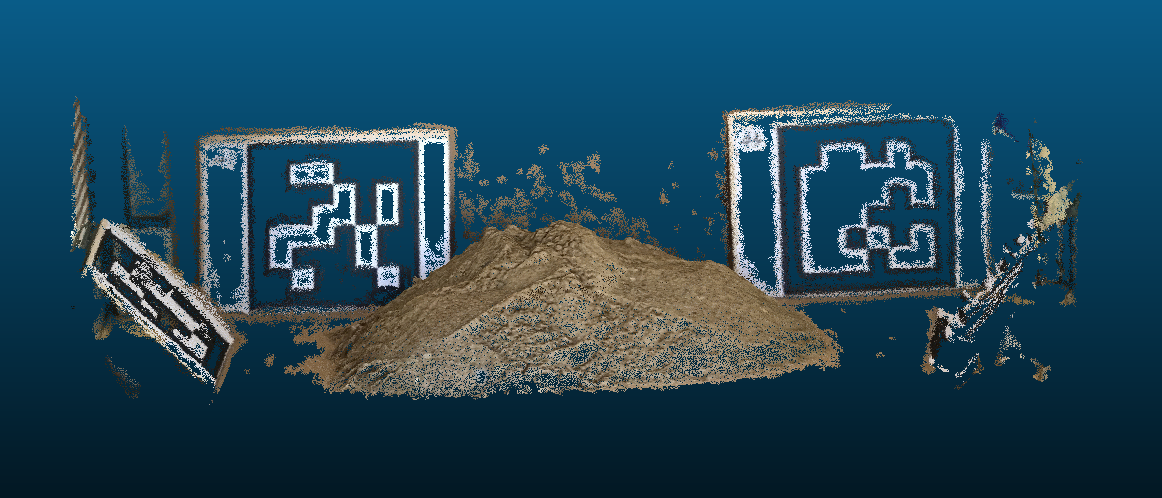
\includegraphics[height=5cm]{5Test_3dconstr_noplane.png}
  \caption{三维重建点云结果示意图}
  \label{fig:5Test_3dconstr_noplane}
  \end{figure}
4.	按照4.2.1节的方式获取2D图像中的角点坐标和对应的三维重建的3D坐标,部分对应关系如表~\ref{tab:chap1:2D_3D}所示。其中最近的2D坐标代表通过三维重建获进行特征点提取时的最近坐标,当3D为-1时,则代表三维重建中的点云没有和该2D图像相对应的3D点。
\begin{table}[h]
  \centering
  \caption{2D坐标和3D坐标关系对应表}
  \label{tab:chap1:2D_3D}
  \begin{tabular}{C{1.6cm}L{2.4cm}L{4.4cm}L{4.4cm}}
  \toprule
  \textbf{图像名称} & \textbf{2D坐标} &\textbf{最近点2D坐标} &  \textbf{3D坐标}  \\
  \midrule
  1613.jpg  &[724, 344]   &[720.478,  343.642]  & -1\\
            &[512, 338]   &[514.977,  337.341]  & [1.75459, -1.35326, 8.97379]\\
  1641.jpg  &[901, 327]   &[902.283,  326.125]  & [3.75985, -1.35022, 8.76246]\\
            &[691, 305]   &[686.783,  313.456]  & [1.74998, -1.29991, 8.97196]\\
  1631.jpg  &[822, 342]   &[825.233,  345.432]  &[3.75985, -1.35022, 8.76246]\\
            &[615, 324]   &[607.253,  323.576]  &[1.69161, -1.38207, 8.97119]\\
  1561.jpg  &[652, 277]   &[649.351,  274.972]  &[3.75985, -1.35022, 8.76246]\\
            &[453, 298]   &[455.467,  297.046]  &[1.75459, -1.35326, 8.97379]\\
  1897.jpg  &[775, 283]   &[775.325,  282.267]  &[3.75985, -1.35022, 8.76246]\\
            &[607, 276]   &[607.673,  276.95]   &[1.75459, -1.35326, 8.97379]\\
  1897.jpg  &[457, 270]   &[461.465,  266.988]  & -1\\
            &[295, 267]   &[296.426,  266.952]  &[-2.24158, -1.3894, 9.26188]\\
  1911.jpg  &[783, 278]   &[780.128,  273.717]  &[3.75985, -1.35022, 8.76246]\\
            &[615, 272]   &[615.711,  273.065]  &[1.75459, -1.35326, 8.97379]\\
  1911.jpg  &[464, 267]   &[463.551,  266.358]  &-1\\
            &[302, 265]   &[303.311,  263.918]  &[-2.24158, -1.3894, 9.26188]\\
  \bottomrule
  \end{tabular}
\end{table}

5. 添加方程:根据4.2.3小节提出的方法,通过上述三维点可以计算出平面方程的参数,可以在原本缺失水平面的点云中按照解析方程添加点云即可,结果如图~\ref{fig:5Test_getVolume_3dconstr}所示,其中红色点云即为水平面。
\begin{figure}[H] % use float package if you want it here
  \centering
  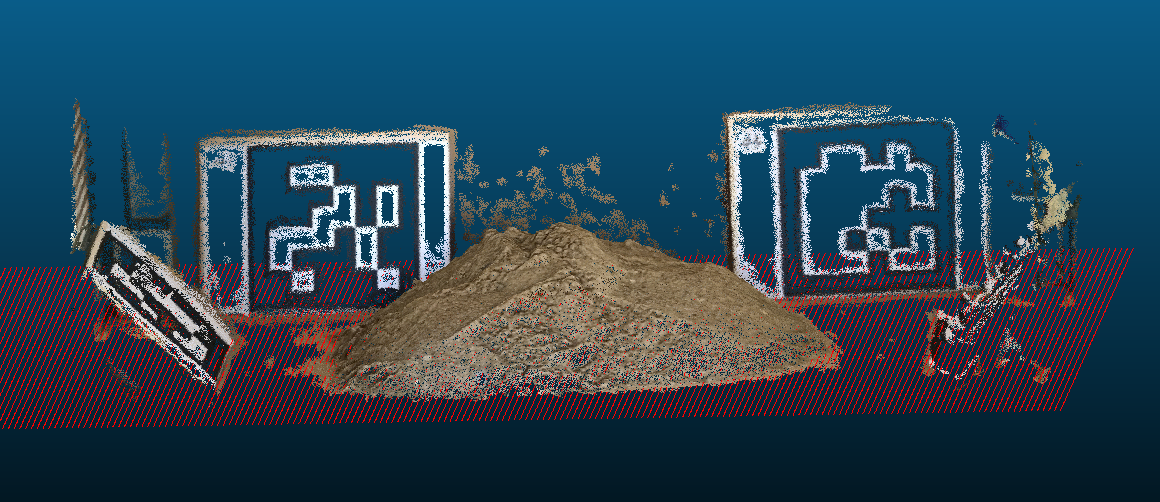
\includegraphics[height=5cm]{5Test_getVolume_3dconstr.png}
  \caption{包含水平面的三维重建结果示意图}
  \label{fig:5Test_getVolume_3dconstr}
  \end{figure}
\subsection{估计堆体实际尺度}
\label{sec:5.4.2}
1. 获取绝对尺度:根据图~\ref{fig:5Test_get_Kabs}所示,分别可以获得在ID = 43的二维码坐标系下的相机位姿,如表~\ref{tab:chap1:2D_3D}前两行,可以计算出在这两帧之间相机移动的绝对距离为0.464m。
\begin{figure}[H] % use float package if you want it here
  \centering
  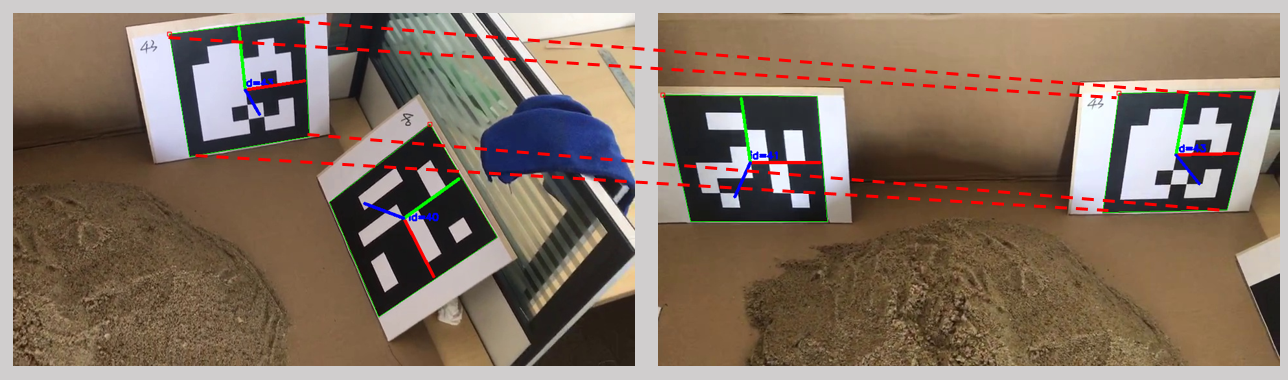
\includegraphics[height=5cm]{5Test_get_Kabs.png}
  \caption{两帧之间获取绝对尺度}
  \label{fig:5Test_get_Kabs}
  \end{figure}
2. 获取相对尺度:从三维重建的结果中提取出这两帧在参考坐标系下的相机位姿,如表~\ref{tab:chap1:2D_3D}后两行,可以计算出这在这两帧之间相机移动的相对距离为4.924。
\begin{table}[h]
  \centering
  \caption{2D坐标和3D坐标关系对应表}
  \label{tab:chap1:2D_3D}
  \begin{tabular}{C{3.6cm}L{2.4cm}L{2.4cm}L{2.4cm}C{3.6cm}}
  \toprule
  \textbf{序号} & \textbf{$T_x$} &\textbf{$T_y$} &  \textbf{$T_z$} &  \textbf{距离} \\
  \midrule
  1027.jpg  &-0.127325& -0.172455& 0.980864& \\
  1167.jpg  &0.324499 &-0.0655995& 0.969803&0.464\\
  1027.jpg  &-6.06873 &1.87705   & -2.13389&         \\
  1167.jpg  &-1.20871 &2.09888   & -1.37369&4.924 \\
  \bottomrule
  \end{tabular}
\end{table}

3. 估计尺度:按照公式~\ref{equ:getVolume_K}通过多组数据优化估计出堆体三维重建和实际堆体之间的尺度因子大小为K = 10.61。
\subsection{堆体体积估计}
针对体积测量实验,本文拟采用如下方式验证所提方法是否能够测量出堆体体积,以及验证测量和测量稳定性。

首先使用测量仪器检测出待测堆体的实际体积真值,随后将堆体分别摆放成单峰堆体,双峰堆体,多峰堆体的形式,如图~\ref{fig:test_1},~\ref{fig:test_2},~\ref{fig:test_3}所示。
按照第~\ref{cha:chap4}章的流程,通过验证三次实验测量值和真值之间的误差衡量视觉算法的精确度,以及对三次测量值之间的数值进行比较,衡量视觉算法测量的稳定性。具体步骤如下:

1. 将某一堆体放置在水平面上,并在堆体周围放置5个二维码以估计尺度和水平面方程。

2. 对上述场景以视频的形式进行图像采集,提取视频中的图像,将数据集的数量控制在200张左右,且每张图像的分辨率在50万左右。

3. 对上述采集到的图像进行二维码检测与识别,记录下每张图像中的二维码ID以及角点坐标。

4. 对上述采集到的图像进行稀疏重建,结果如图~\ref{fig:test_1_sparse},~\ref{fig:test_2_sparse},~\ref{fig:test_3_sparse},所示,记录下稀疏点云中的3D点和每张图像角点之间的映射关系。

5. 按照~\ref{sec:4.2}估计堆体出水平面方程。

6. 按照~\ref{sec:4.3}估计出堆体的尺度大小。

7. 对稀疏点云进行稠密重建,结果如图~\ref{fig:test_1_dense},~\ref{fig:test_2_dense},~\ref{fig:test_3_dense}所示,并将所求解出的水平面方程添加至稠密点云中。

8. 按照~\ref{sec:4.4}估计出当前堆体的体积大小。

9. 将单个堆体分别设计成2个堆体和3个堆体的情况,重复步骤2$~$8,计算不同场景对应的体积。

10 根据结果定量分析上述视觉算法测量堆体的准确性和稳定性。

3次实验结果如表~\ref{tab:volume_test}所示。
\begin{table}[h]
  \centering
  \caption{体积测量结果}
  \label{tab:volume_test}
  \begin{tabular}{C{1.1cm}C{1.2cm}C{1.2cm}C{1.2cm}C{3.6cm}C{1.6cm}C{1.6cm}C{1.5cm}}
  \toprule
  \textbf{批次} & \textbf{图像数} & \textbf{点个数}& \textbf{尺度K} & \textbf{水平面方程}& \textbf{计算耗时(s)} & \textbf{堆体体积($cm^3$)} & \textbf{测量精度}\\
  \midrule
  1 & 186  &110149 &1.945 &-0.0259x-0.0331y-0.0873z+1=0 & 712 & 13221.4  &   1.7$\%$\\
  2 & 201  & 86403 &8.143 &0.0068x-0.0299y-0.0620z+1=0  & 675 & 12758.3  &   1.8$\%$\\
  3 & 215  & 83196 &3.522 &0.0119x-0.0254y-0.0683z+1=0  & 663 & 12830.2  &   1.3$\%$\\
  \bottomrule
\end{tabular}
\end{table}

对上述沙堆使用仪器测量出的体积真值为13000$cm^3$,通过三次实验,分别得出测量单峰堆体,双峰堆体,多峰堆体的体积
为13221.4$cm^3$,12758.3$cm^3$,12830.2$cm^3$,测量的误差可以控制在2$\%$以内,且三次测量值接近,测量稳定。

\begin{figure}[H]
  \centering
  \subcaptionbox{单峰预览图\label{fig:test_1}}{
  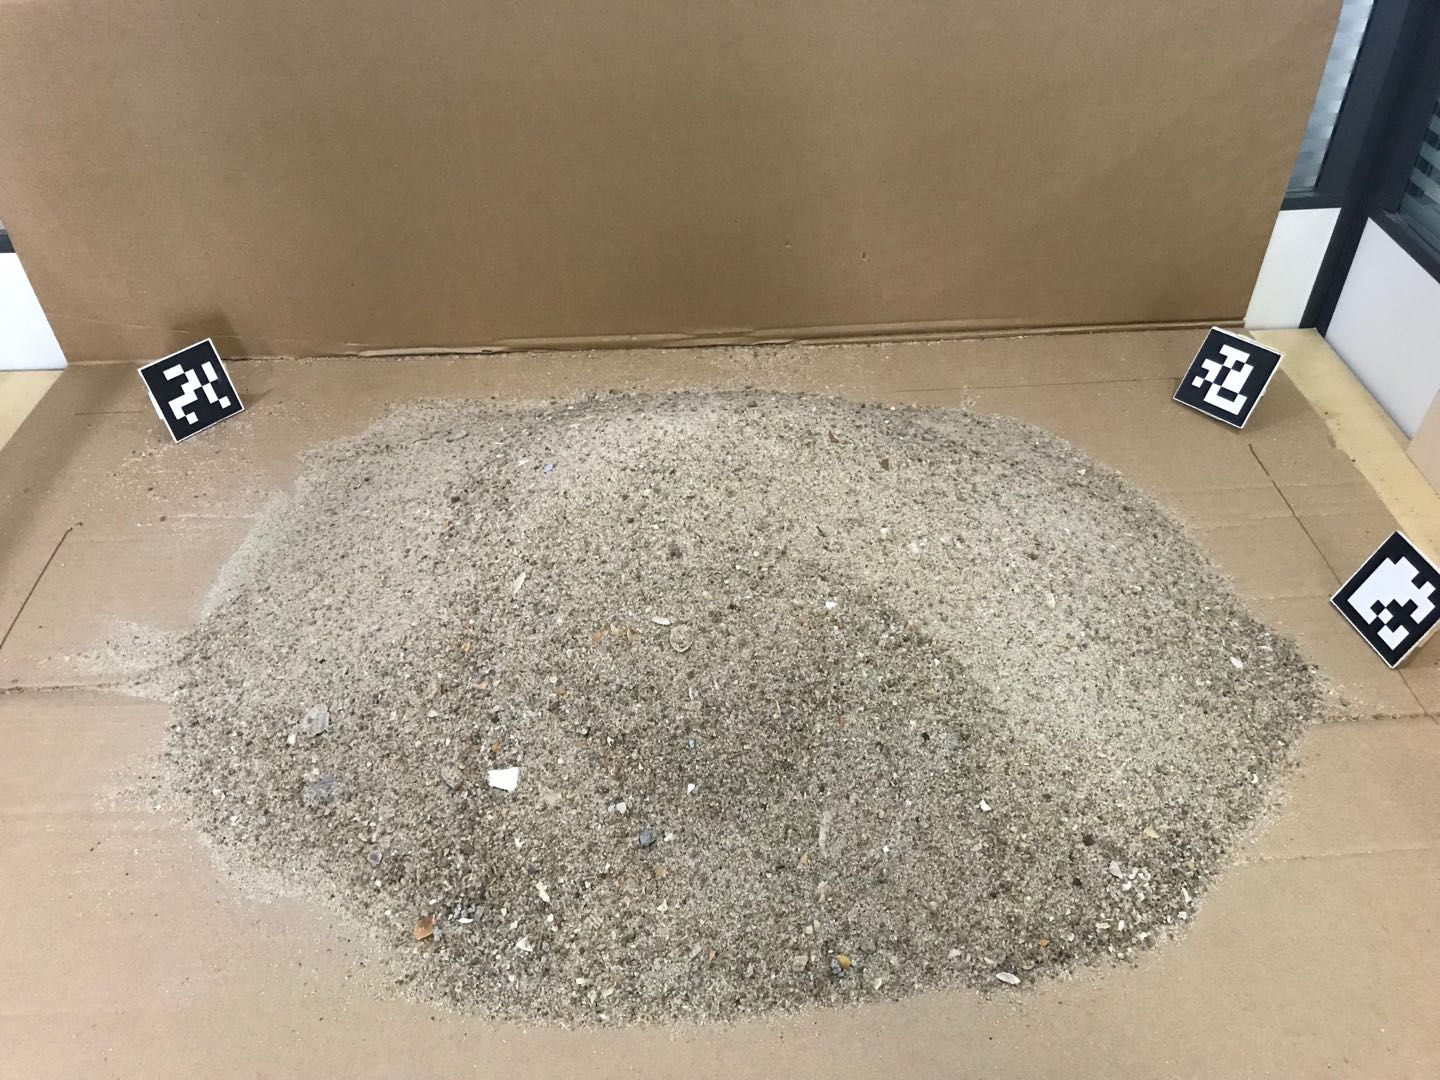
\includegraphics[width=6.5cm,height=4.2cm,angle=90]{test_1.png}\hskip0.5cm}
  \subcaptionbox{单峰稀疏点云图\label{fig:test_1_sparse}}{
  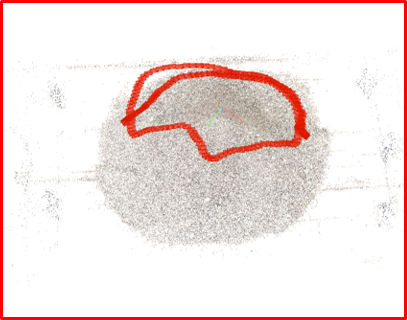
\includegraphics[width=6.5cm,height=4.2cm,angle=90]{test_1_sparse.png}\hskip0.5cm}
  \subcaptionbox{单峰稠密点云图\label{fig:test_1_dense}}{
  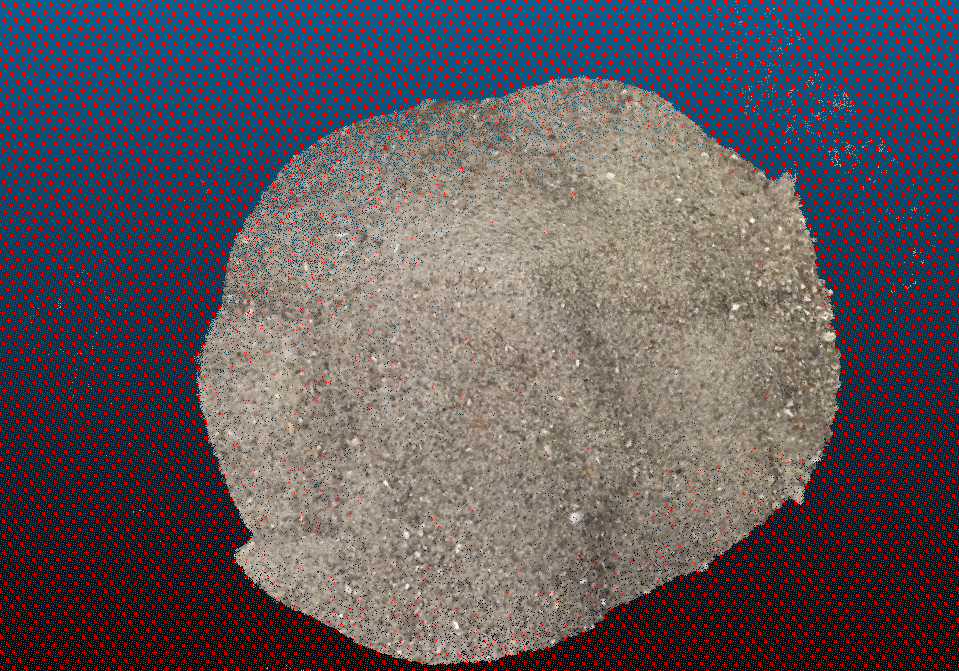
\includegraphics[width=6.5cm,height=4.2cm,angle=90]{test_1_dense.png}}
\vskip0.2cm
   \subcaptionbox{双峰预览图\label{fig:test_2}}{
  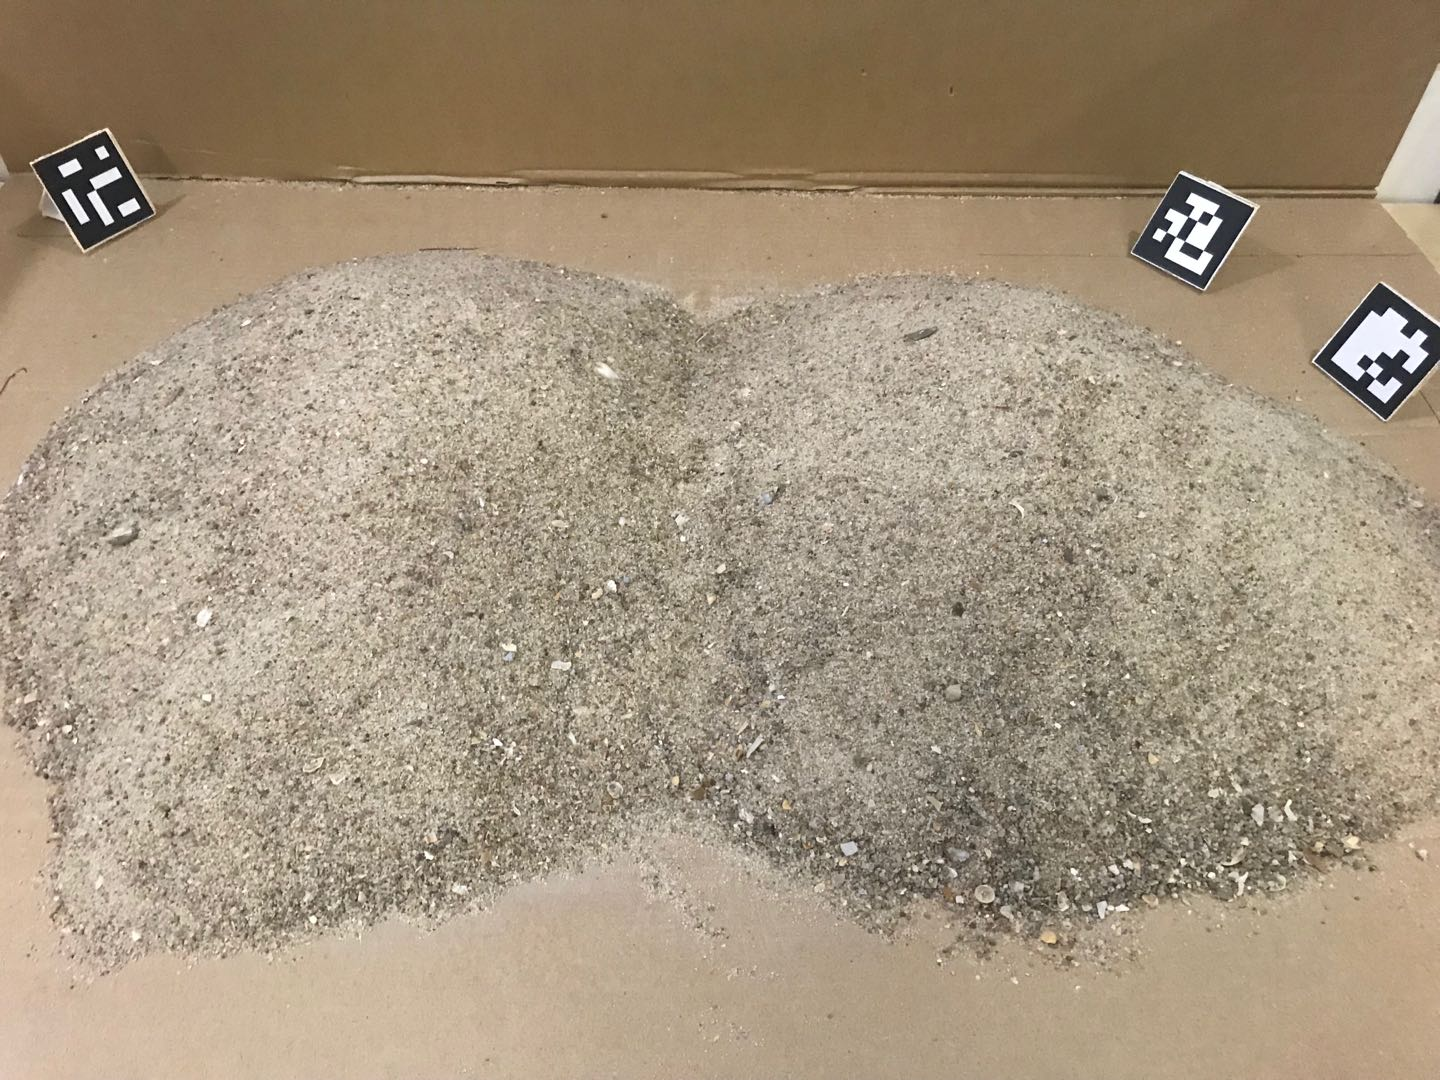
\includegraphics[width=6.5cm,height=4.2cm,angle=90]{test_2.png}\hskip0.5cm}
  \subcaptionbox{双峰稀疏点云图\label{fig:test_2_sparse}}{
  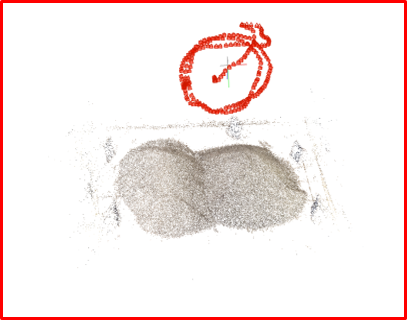
\includegraphics[width=6.5cm,height=4.2cm,angle=90]{test_2_sparse.png}\hskip0.5cm}
  \subcaptionbox{双峰稠密点云图\label{fig:test_2_dense}}{
  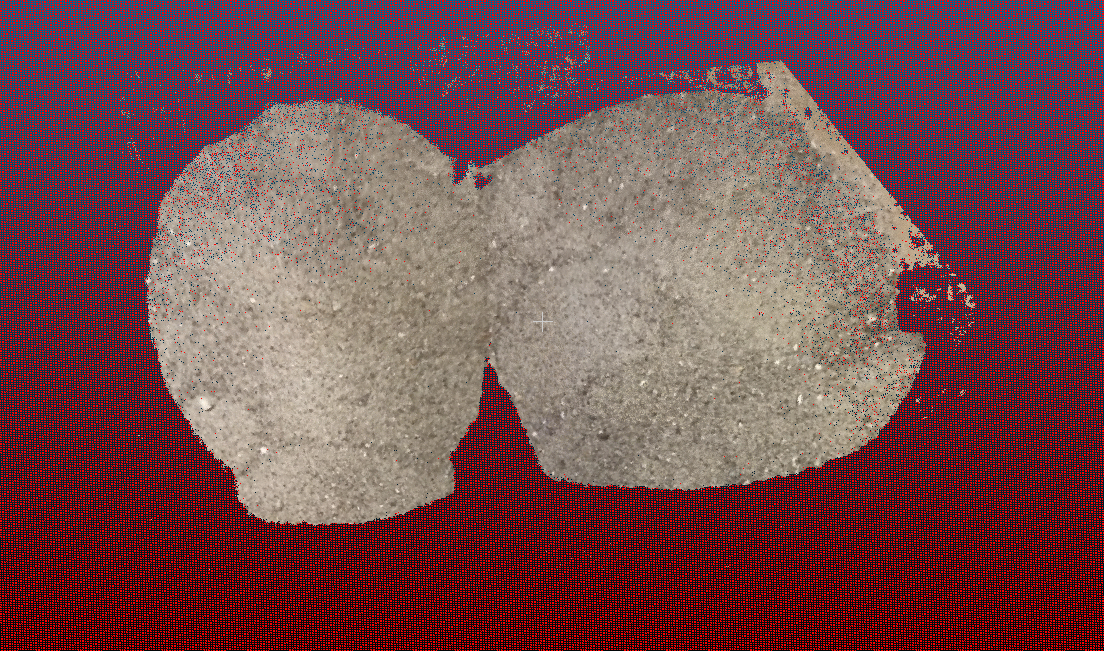
\includegraphics[width=6.5cm,height=4.2cm,angle=90]{test_2_dense.png}}
\vskip0.2cm      
   \subcaptionbox{多峰预览图\label{fig:test_3}}{
  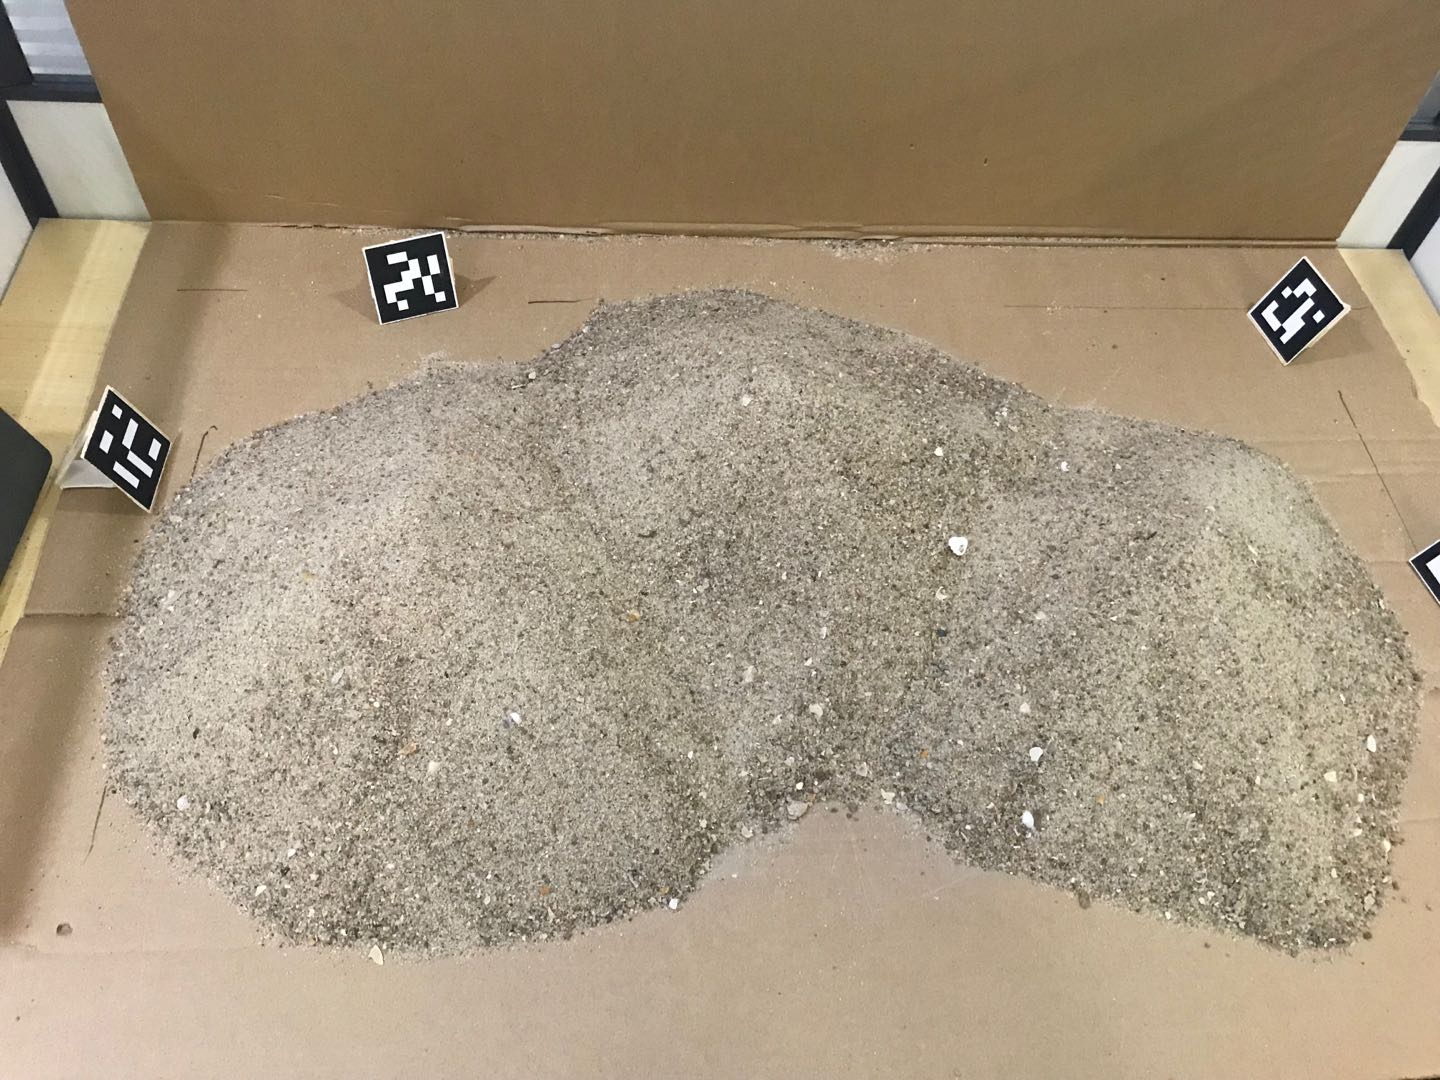
\includegraphics[width=6.5cm,height=4.2cm,angle=90]{test_3.png}\hskip0.5cm}
  \subcaptionbox{多峰稀疏点云图\label{fig:test_3_sparse}}{
  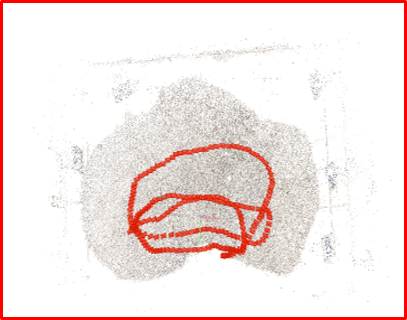
\includegraphics[width=6.5cm,height=4.2cm,angle=90]{test_3_sparse.png}\hskip0.5cm}
  \subcaptionbox{多峰稠密点云图\label{fig:test_3_dense}}{
  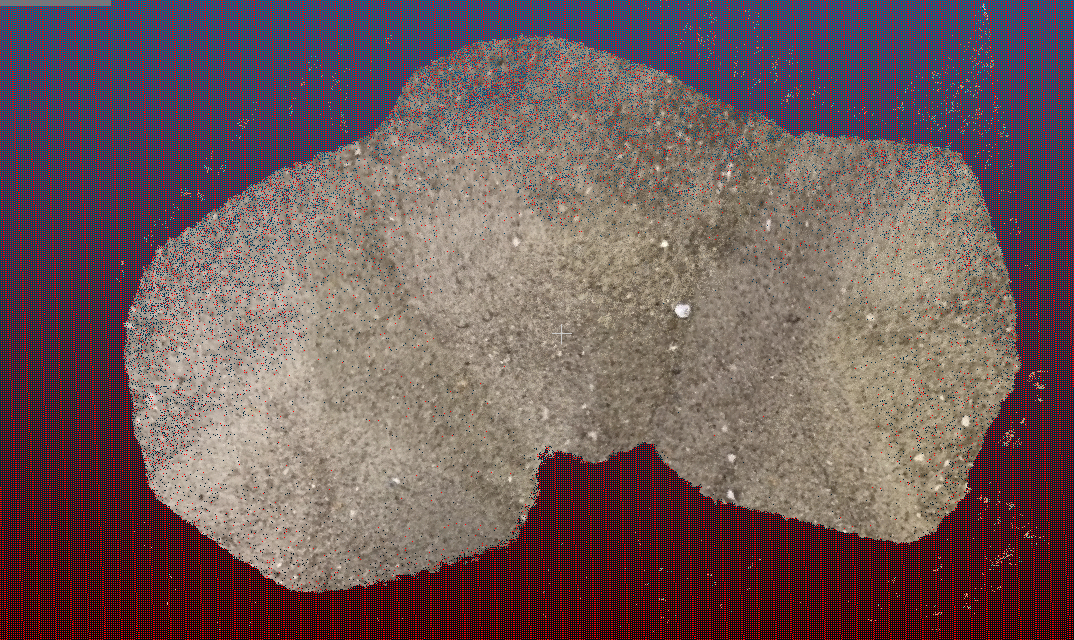
\includegraphics[width=6.5cm,height=4.2cm,angle=90]{test_3_dense.png}}

\caption{多类别堆体示意图}\label{fig:2VSLAM_big}
\end{figure}

% \begin{sidewaysfigure}
%   \centering
%   \subcaptionbox{x轴旋转\label{fig:chap05:rx}}{
%   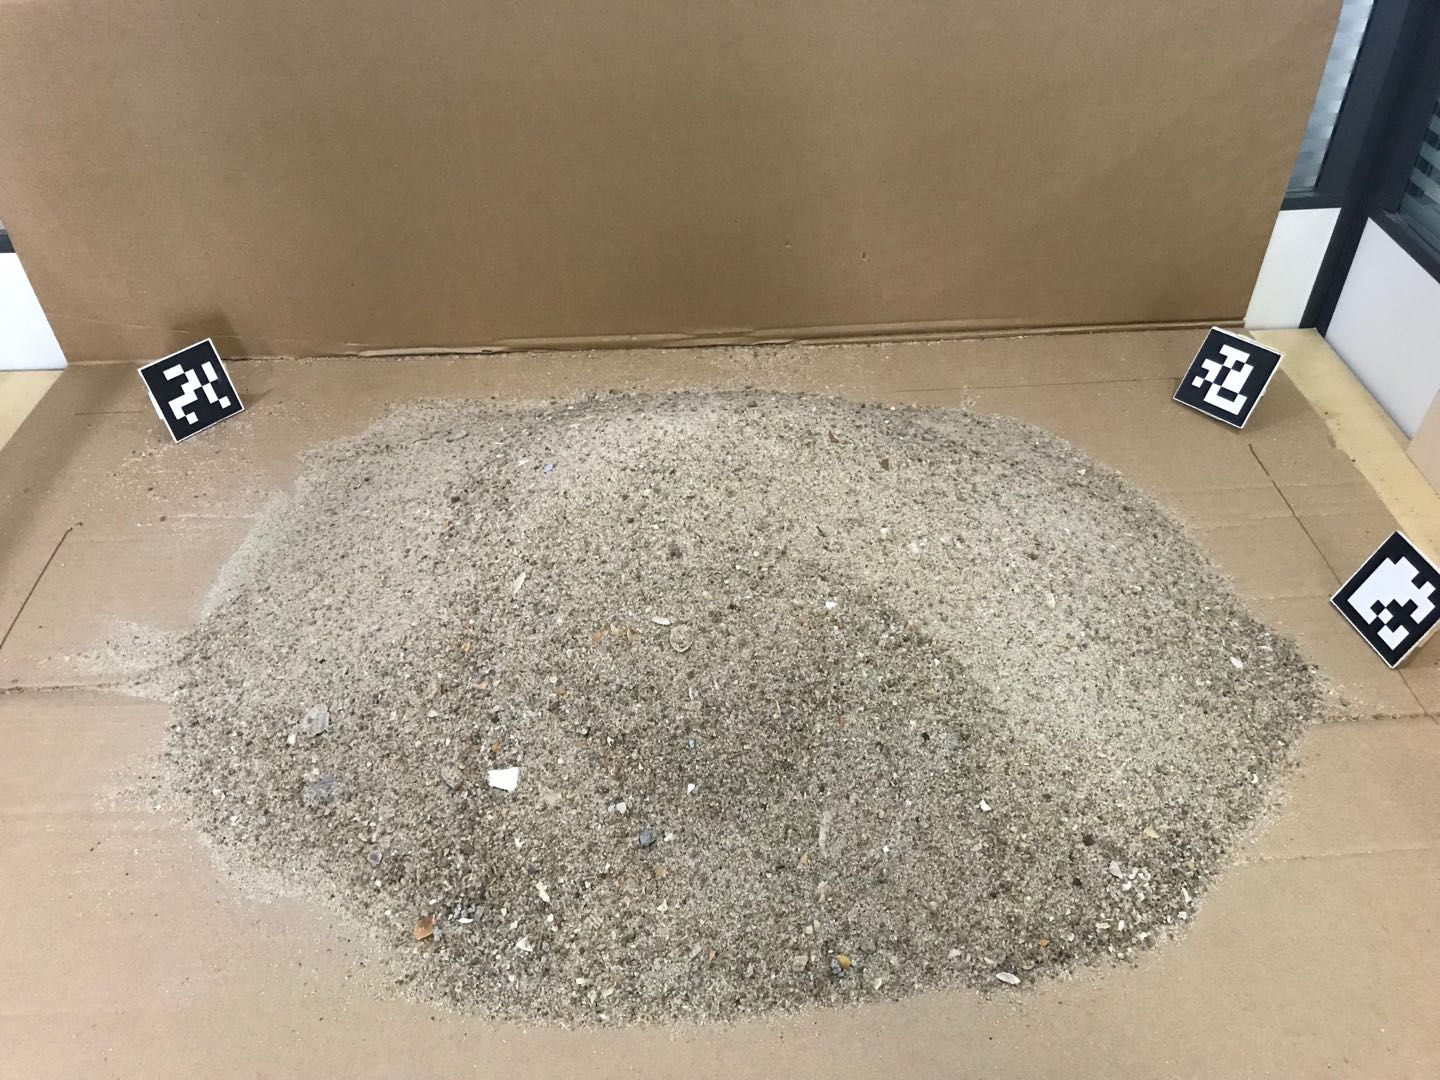
\includegraphics[width=0.31\textwidth]{test_1.png}}\hspace{0.1em}
%   \subcaptionbox{y轴旋转\label{fig:chap05:ry}}{
%   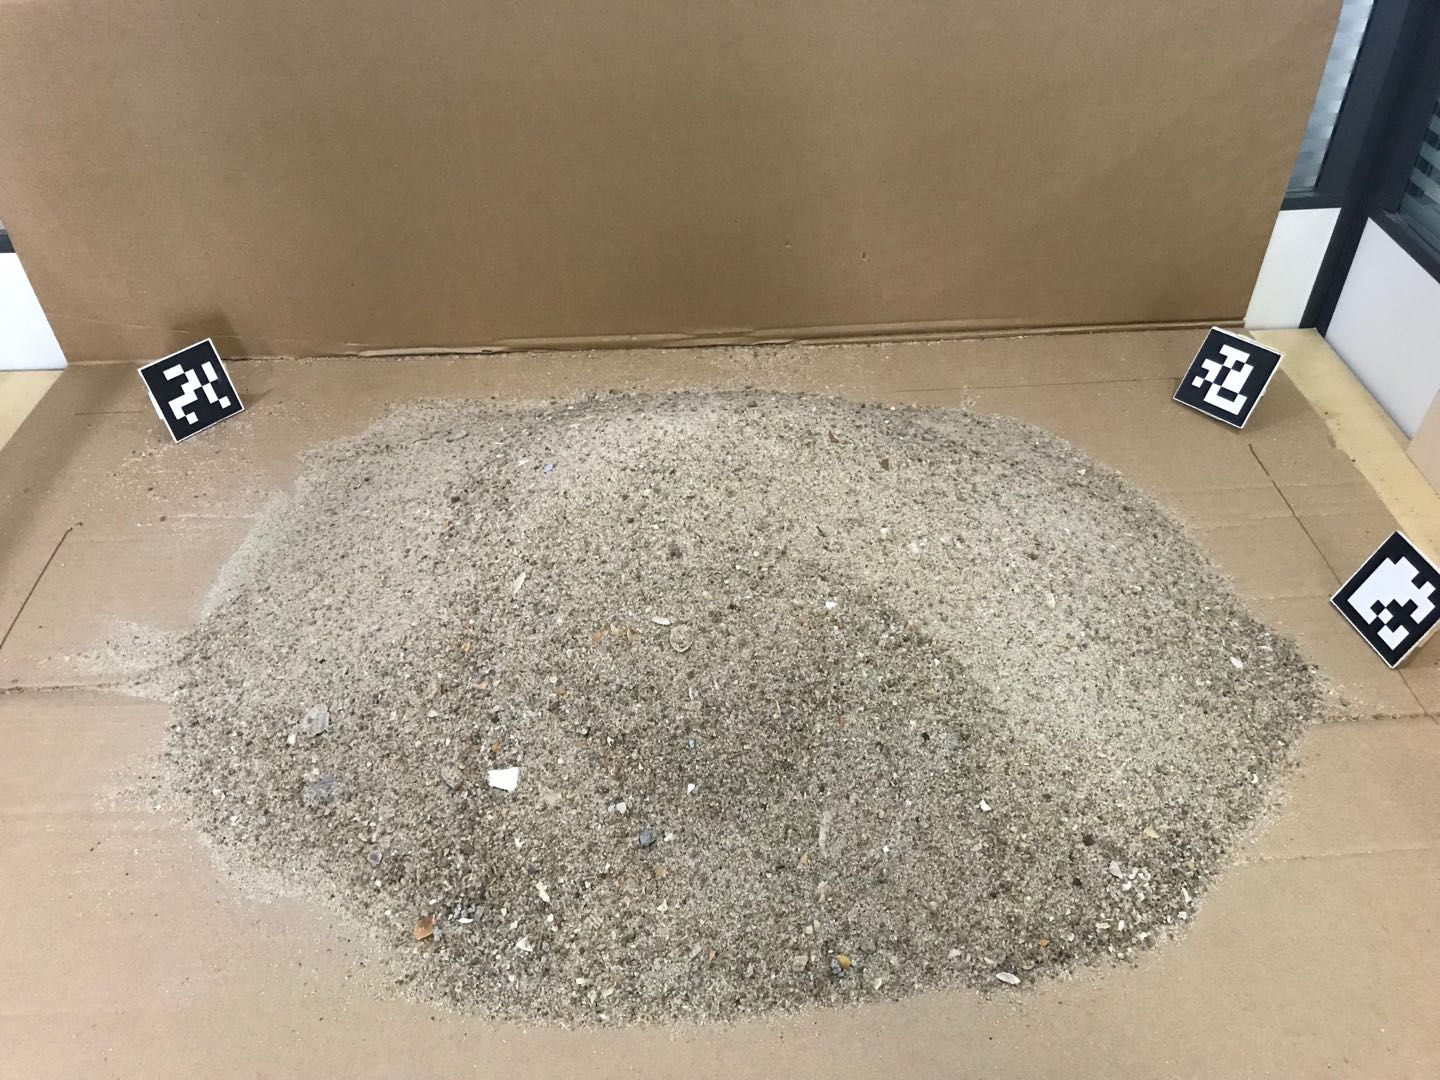
\includegraphics[width=0.31\textwidth]{test_1.png}}\hspace{0.1em}
%   \subcaptionbox{z轴旋转\label{fig:chap05:rz}}{
%   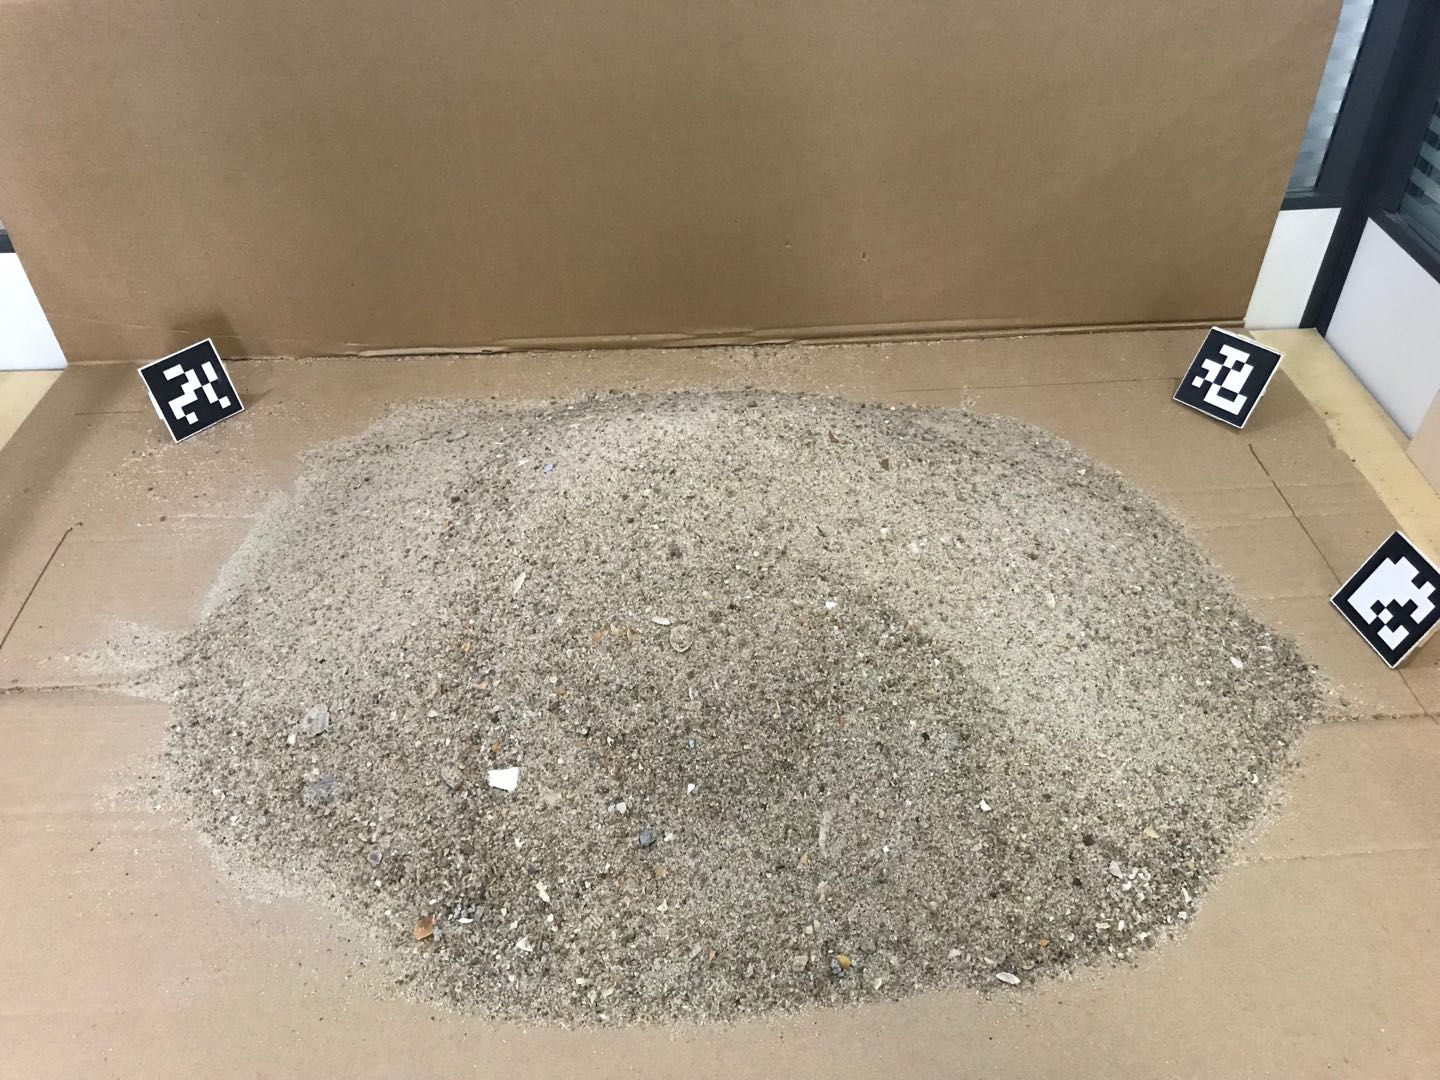
\includegraphics[width=0.31\textwidth]{test_1.png}}
%   \vskip 0.3cm
%   \subcaptionbox{x轴平移\label{fig:chap05:tx}}{
%   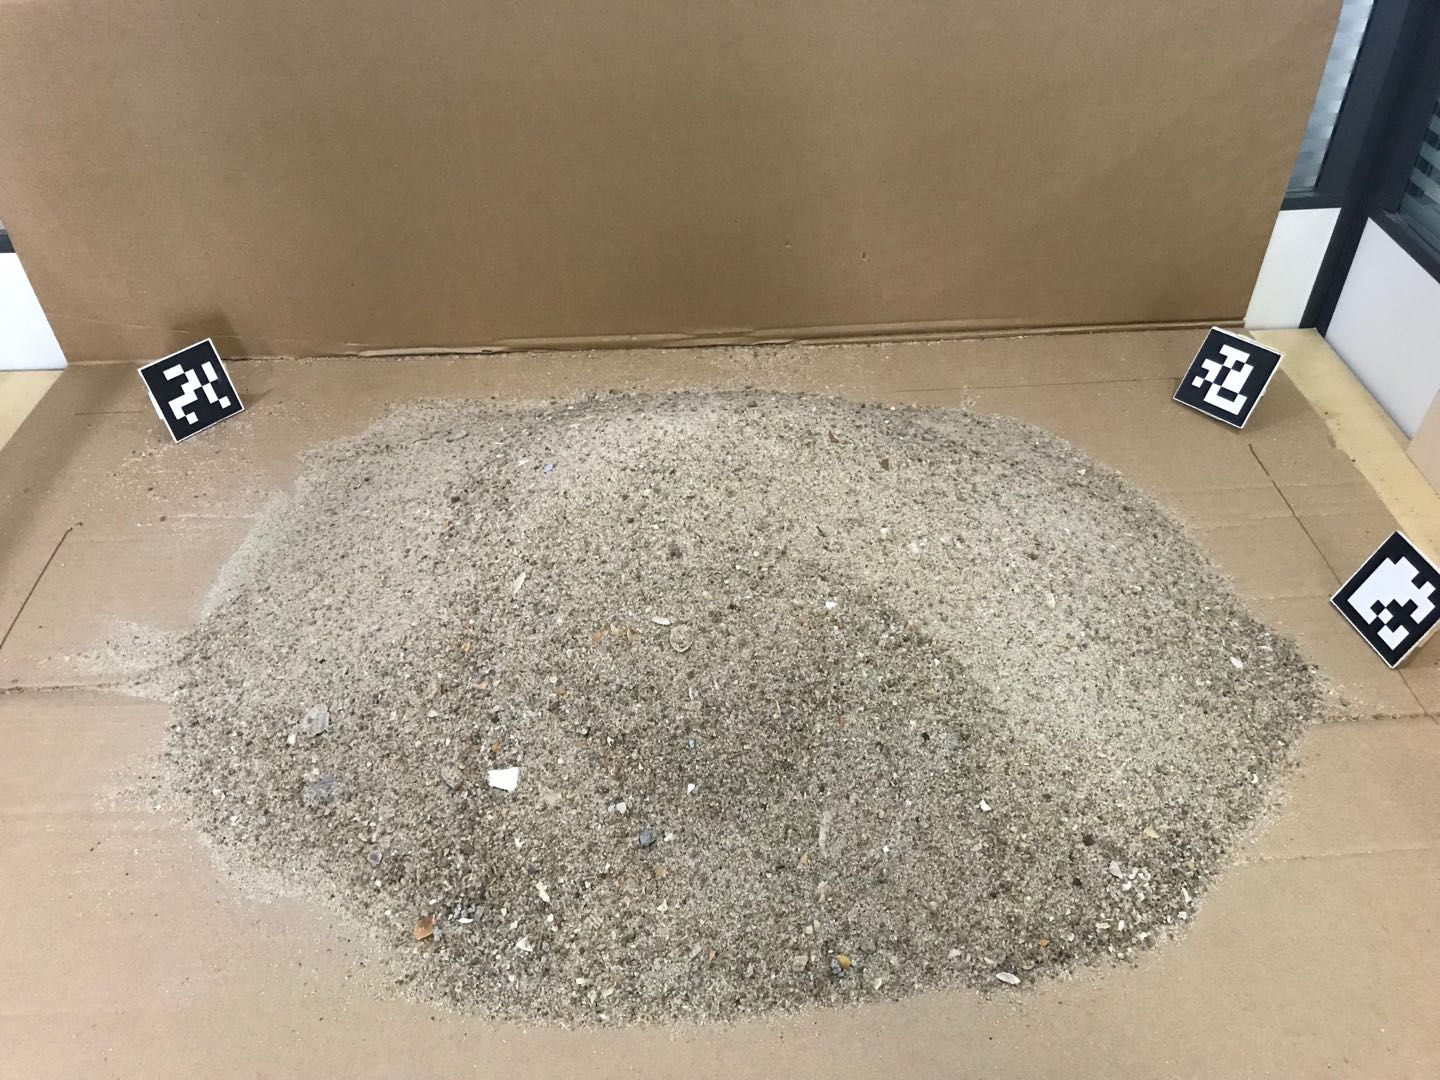
\includegraphics[width=0.31\textwidth]{test_1.png}}\hspace{0.1em}
%   \subcaptionbox{y轴平移\label{fig:chap05:ty}}{
%   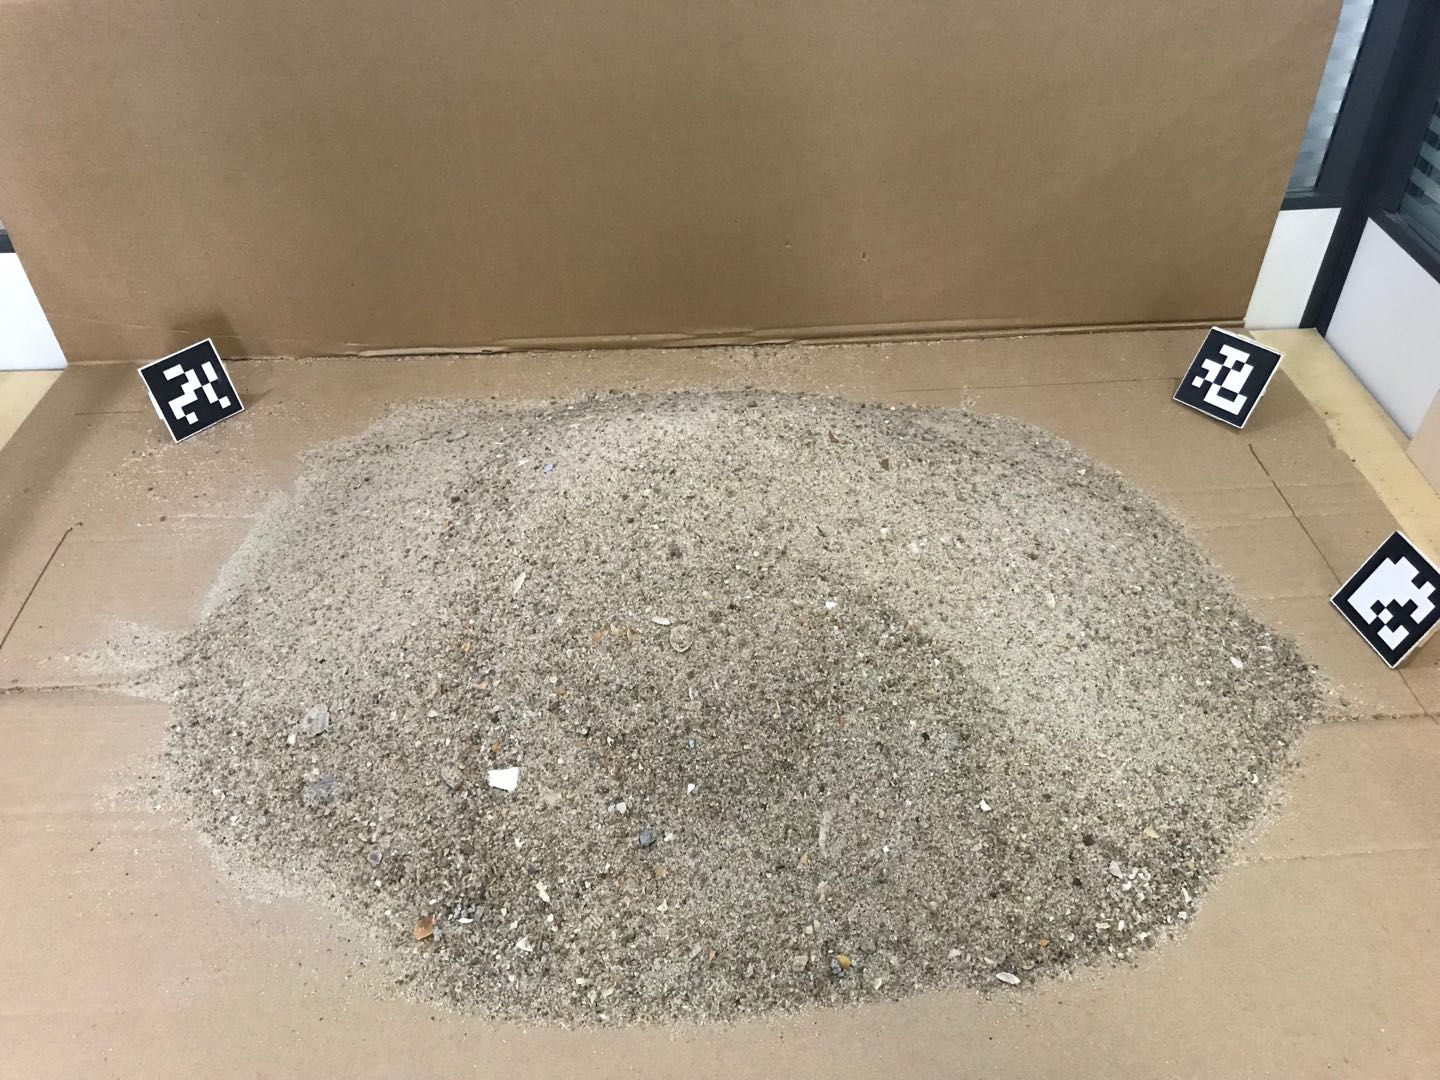
\includegraphics[width=0.31\textwidth]{test_1.png}}\hspace{0.1em}
%   \subcaptionbox{z轴平移\label{fig:chap05:tz}}{
%   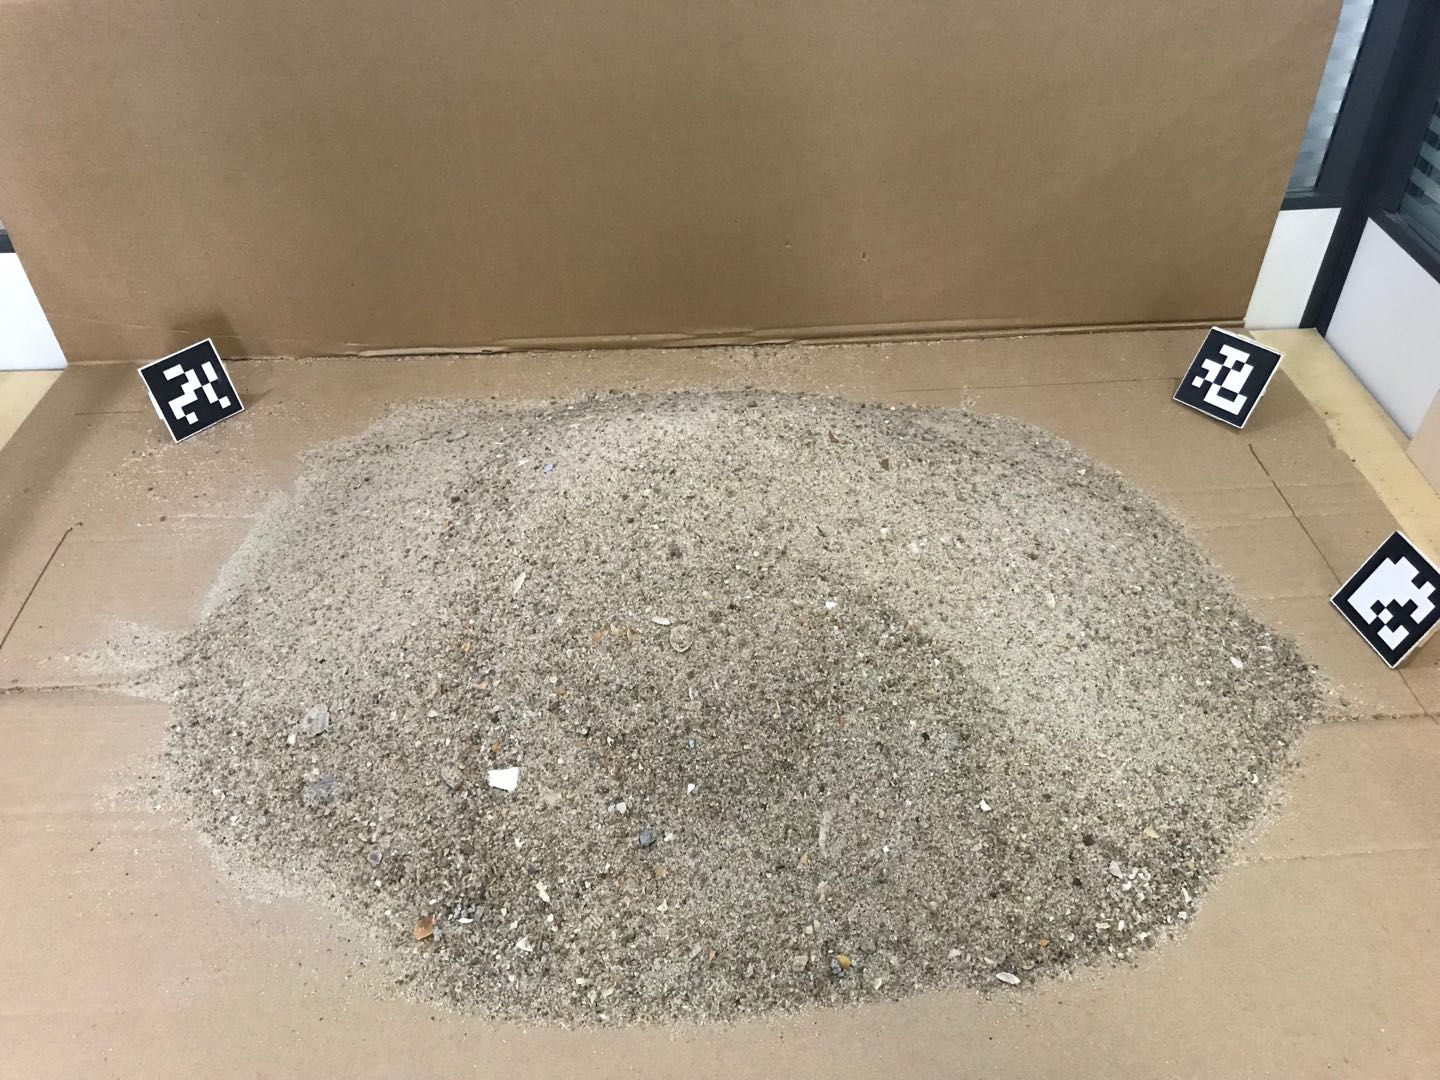
\includegraphics[width=0.31\textwidth]{test_1.png}}
%   \caption{Rigid Pose追踪精度测试图}
%   \label{fig:chap05:rigidpose_rig_track}
% \end{sidewaysfigure}

% \begin{figure}[h]
%   \centering
%       \subcaptionbox{单峰预览图\label{fig:2VSLAM_big1}}{
%       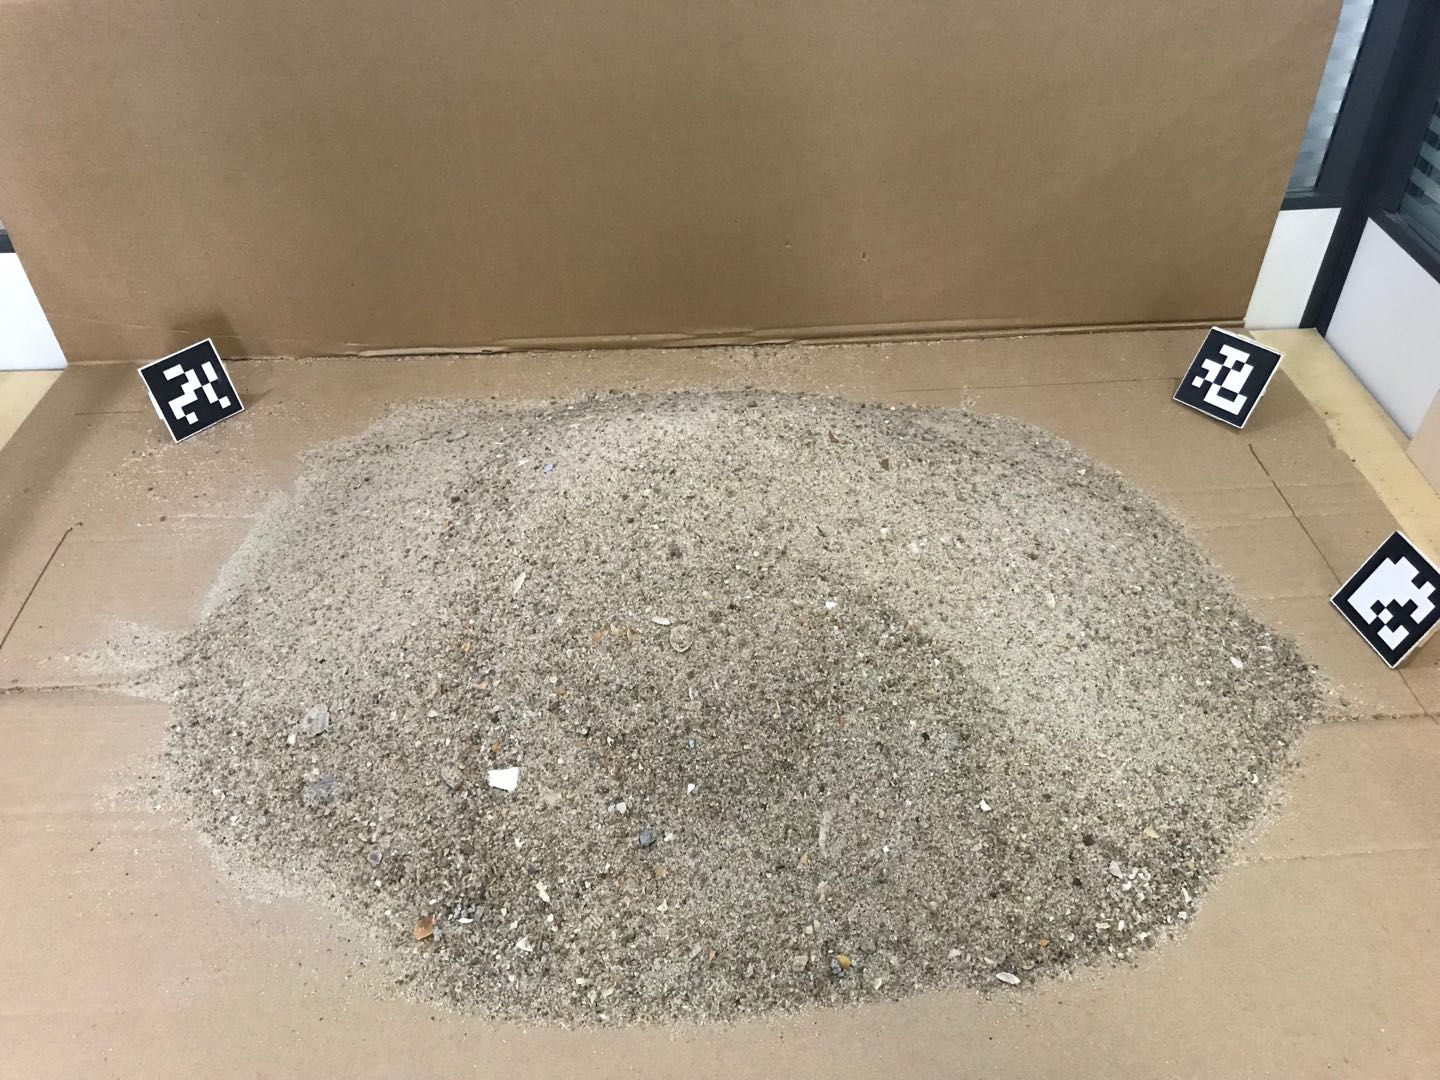
\includegraphics[width=4cm]{test_1.png}\hskip1cm}
%       \subcaptionbox{双峰预览图\label{fig:2VSLAM_big2}}{
%       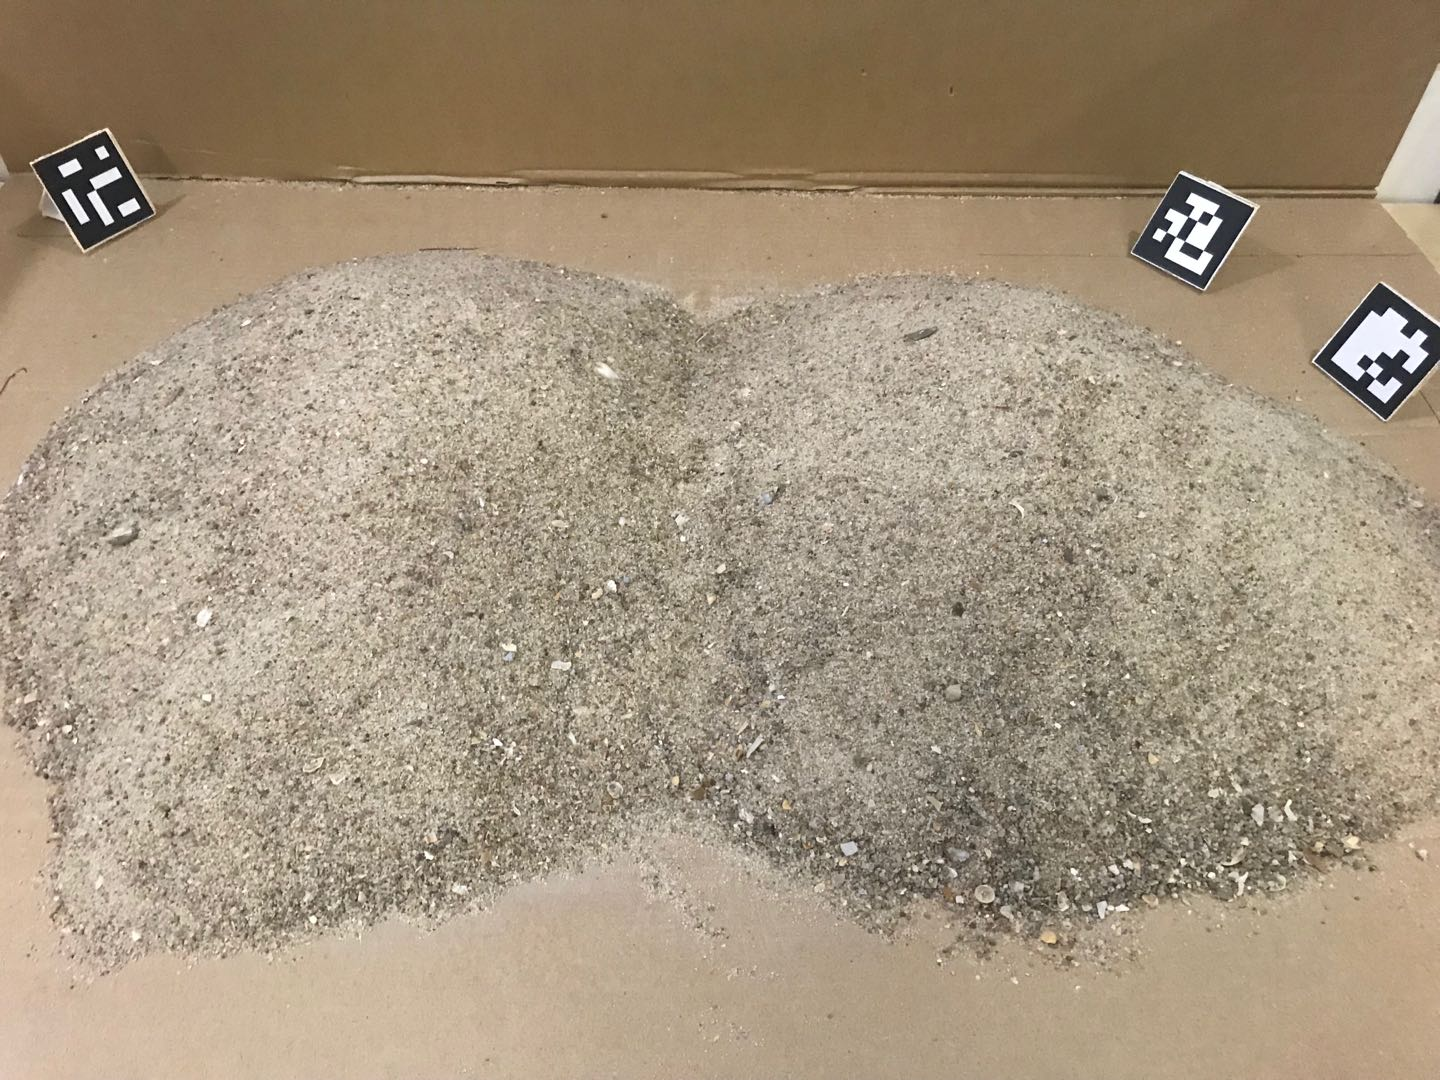
\includegraphics[width=4cm]{test_2.png}\hskip1cm}
%       \subcaptionbox{多峰预览图\label{fig:2VSLAM_big2}}{
%       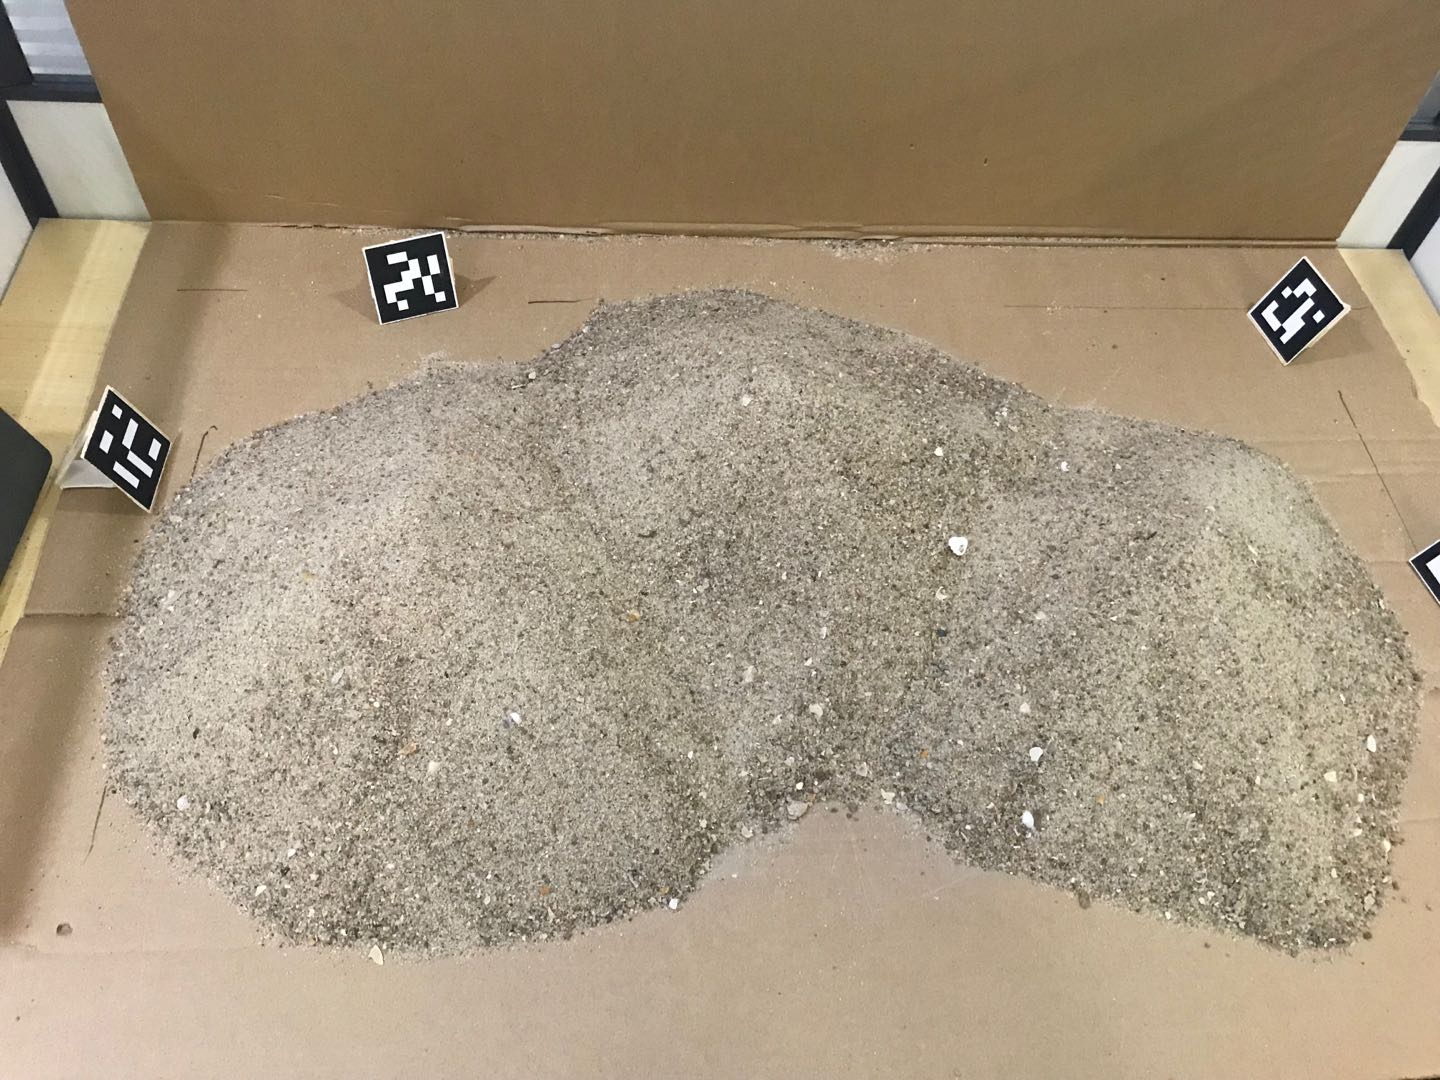
\includegraphics[width=4cm]{test_3.png}}
%     \vskip0.2cm
%       \subcaptionbox{单峰稀疏点云图\label{fig:2VSLAM_big4}}{
%       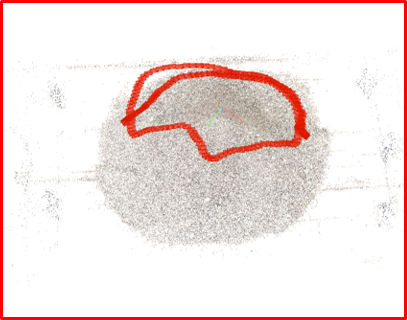
\includegraphics[width=4cm]{test_1_sparse.png}\hskip1cm}
%       \subcaptionbox{双峰稀疏点云图\label{fig:2VSLAM_big5}}{
%       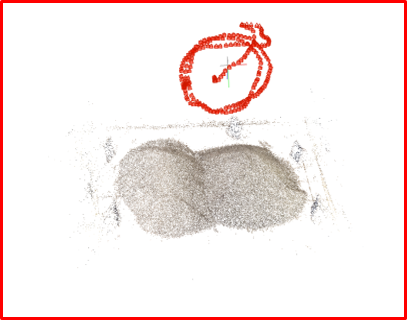
\includegraphics[width=4cm]{test_2_sparse.png}\hskip1cm}
%       \subcaptionbox{多峰稠密点云图\label{fig:2VSLAM_big6}}{
%       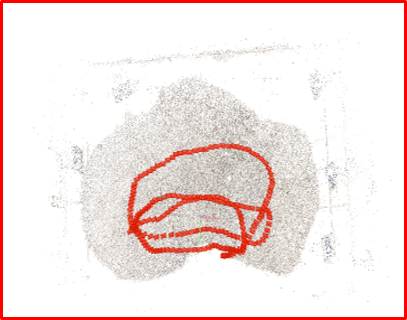
\includegraphics[width=4cm]{test_3_sparse.png}}
%     \vskip0.2cm      
%       \subcaptionbox{单峰稠密点云图\label{fig:2VSLAM_big7}}{
%       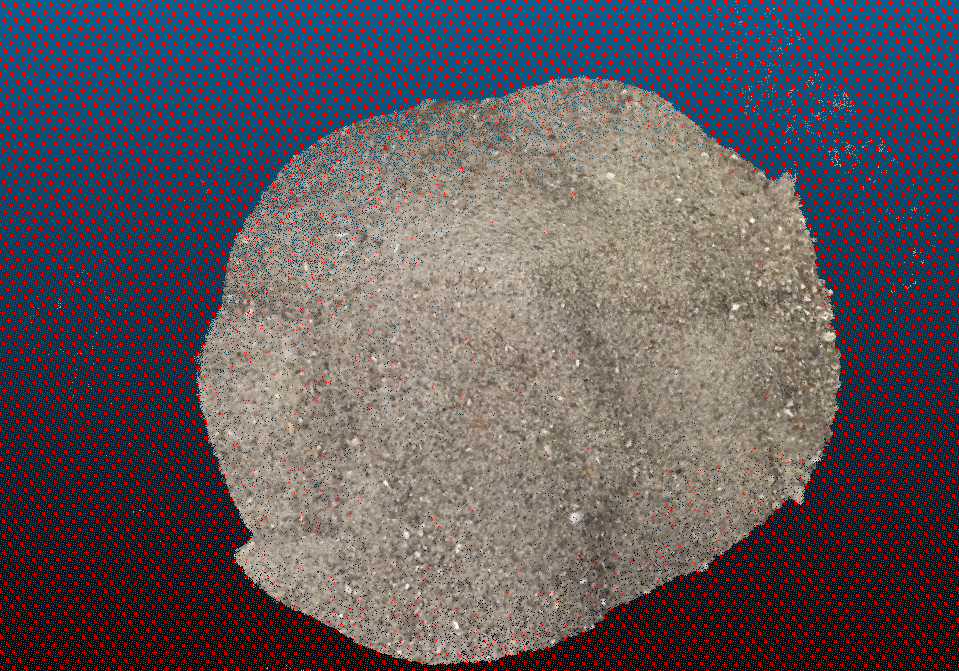
\includegraphics[width=4cm]{test_1_dense.png}\hskip1cm}
%       \subcaptionbox{双峰稠密点云图\label{fig:2VSLAM_big8}}{
%       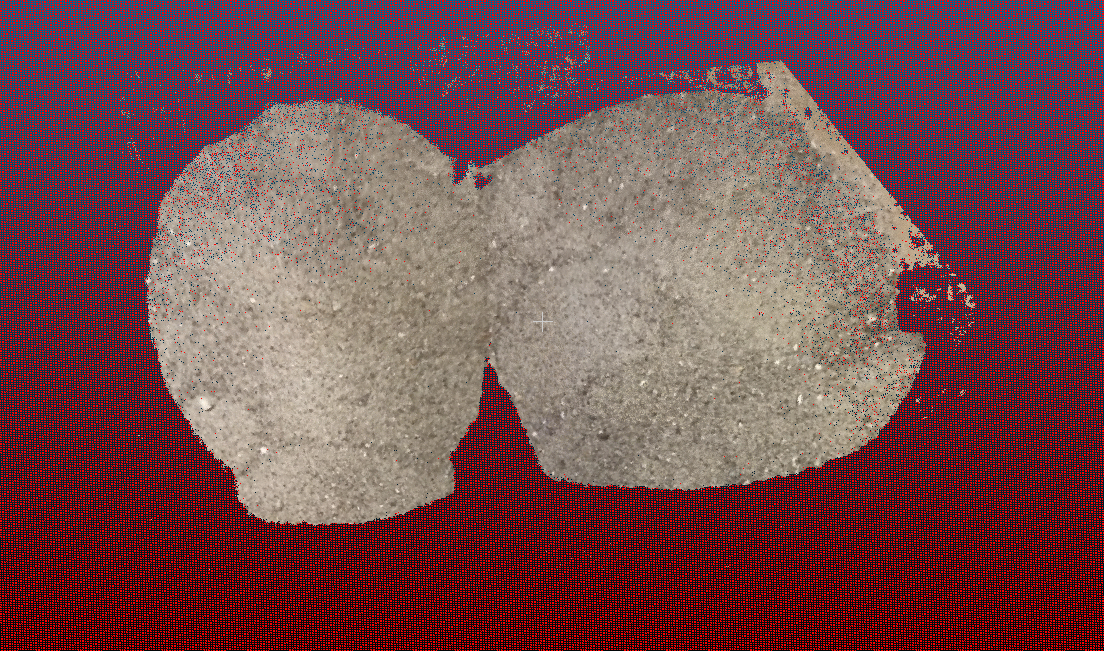
\includegraphics[width=4cm]{test_2_dense.png}\hskip1cm}
%       \subcaptionbox{多峰稀疏点云图\label{fig:2VSLAM_big9}}{
%       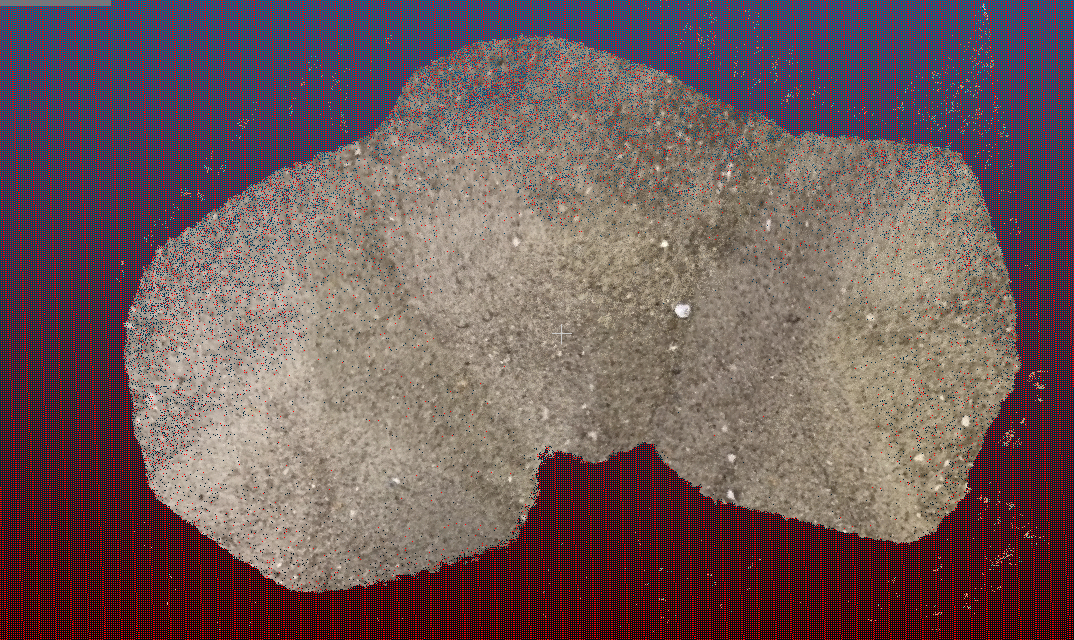
\includegraphics[width=4cm]{test_3_dense.png}}

%   \caption{多类别堆体示意图}\label{fig:2VSLAM_big}
% \end{figure}
% \begin{table}[]
%   \centering
%   \caption{体积测量结果-\uppercase\expandafter{\romannumeral1}}
%   \label{tab:volume_test_1}
%   \begin{tabular}{C{2.4cm}C{2.0cm}C{8.0cm}C{2cm}}
%   \toprule
%   \textbf{实验批次} & \textbf{图像集数量} & \textbf{堆体场景预览} & \textbf{图像分辨率} \\
%   \midrule
%   1 & 186   & 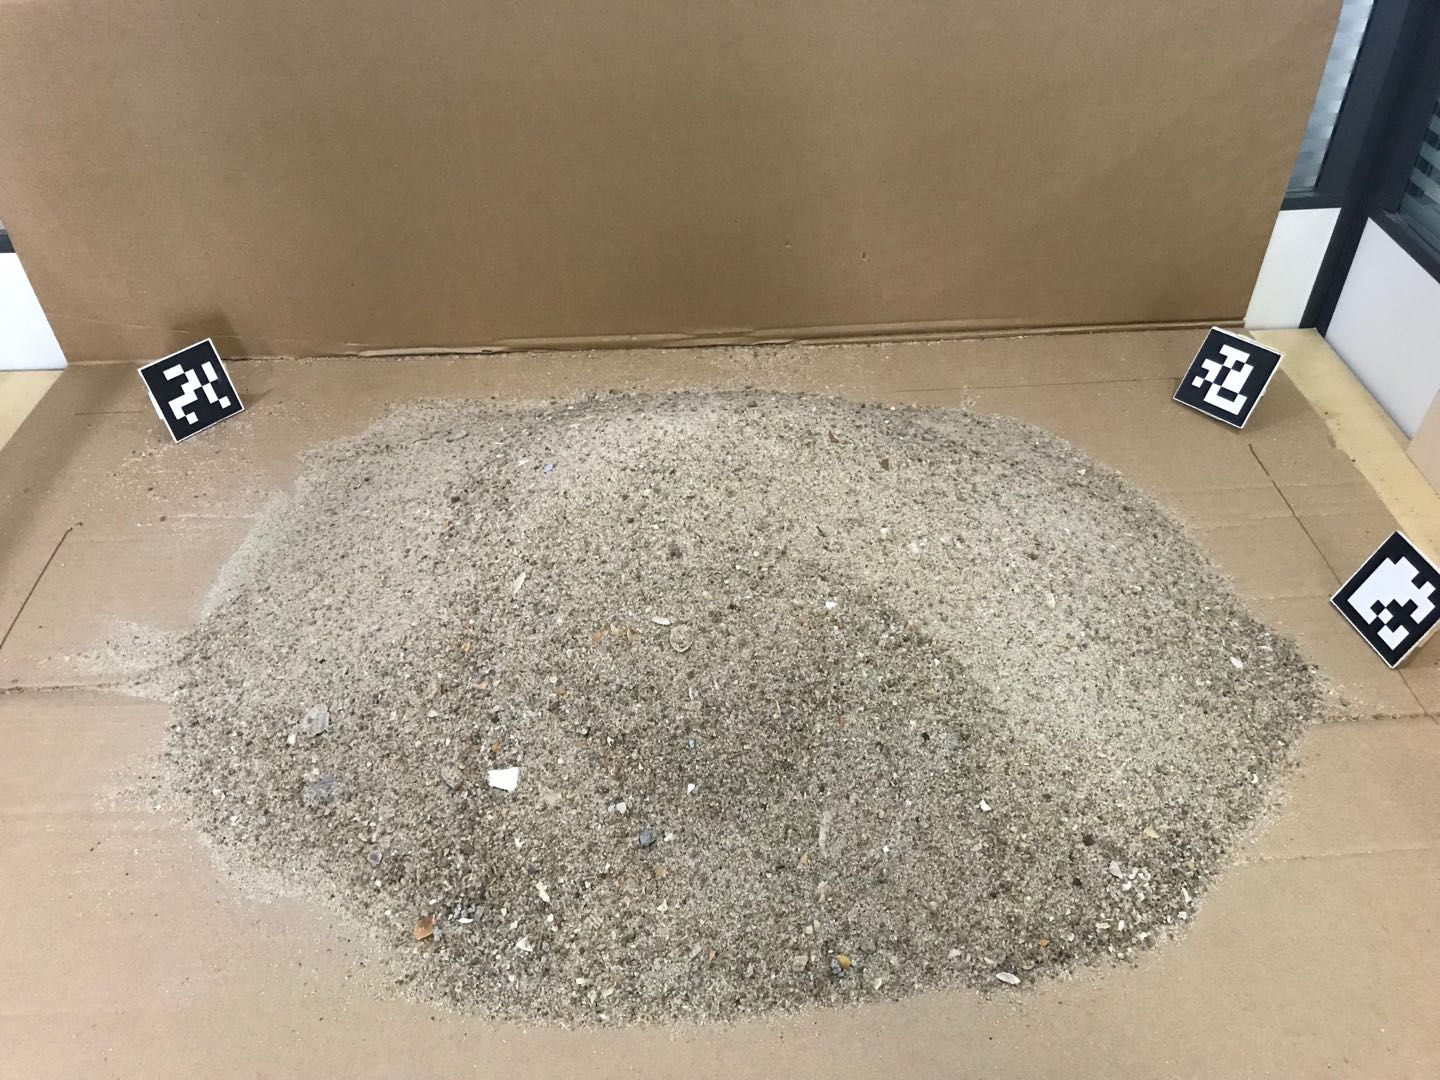
\includegraphics[width=7.5cm, height=5cm]{test_1.png} & 960*455 \\
%   2 & 201   & 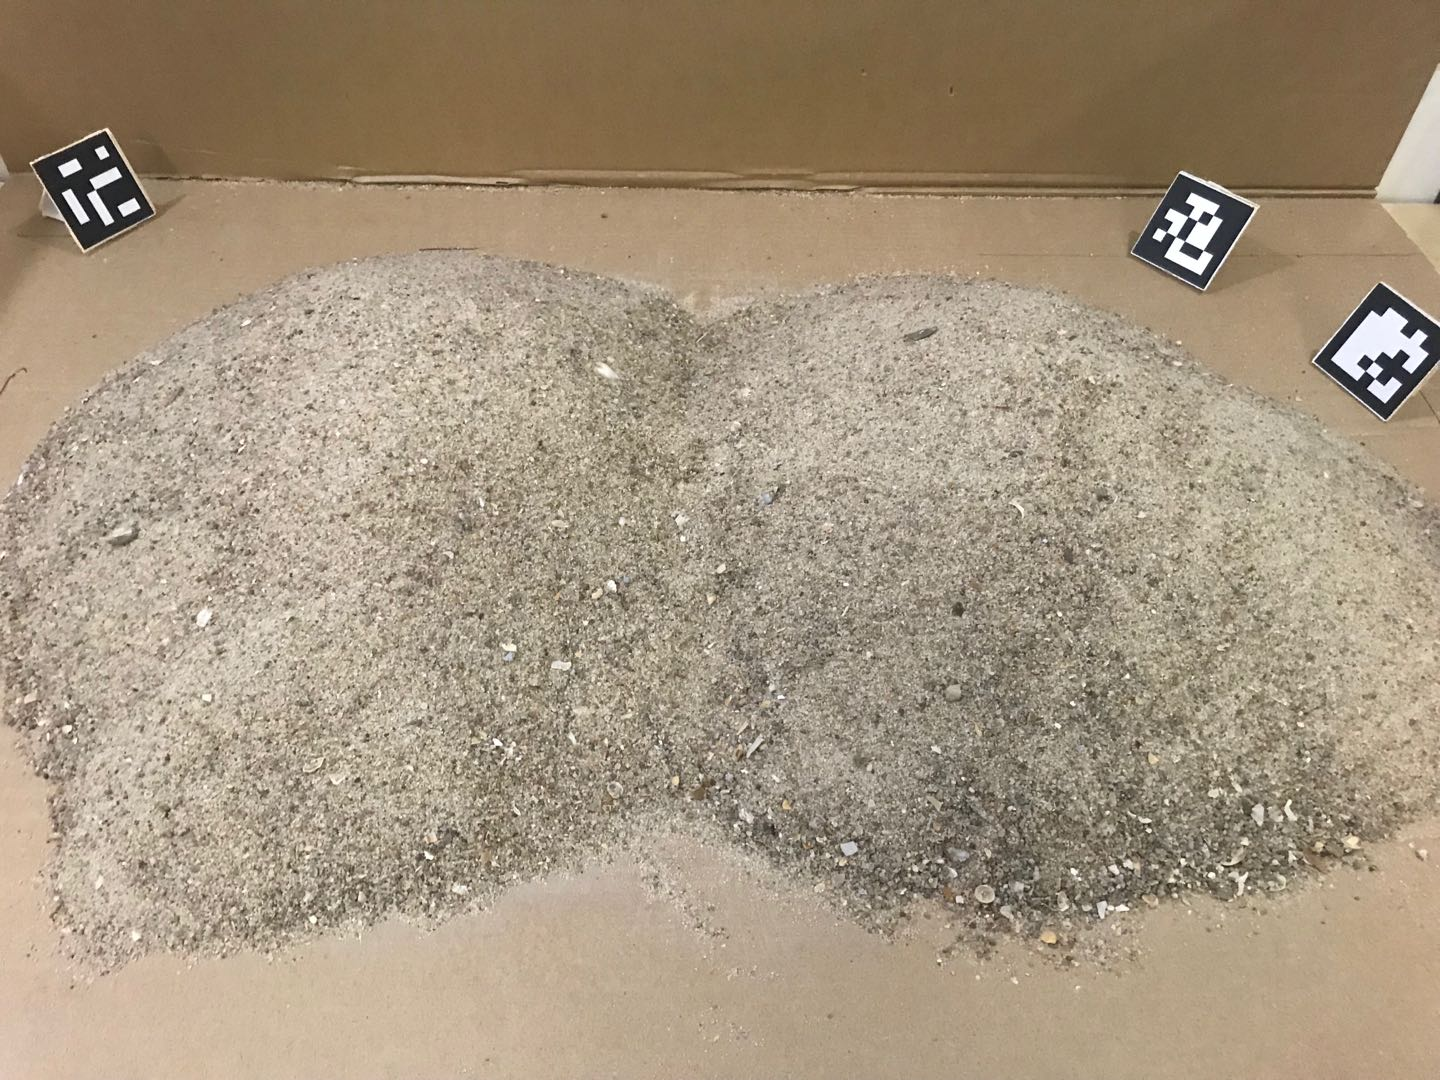
\includegraphics[width=7.5cm, height=5cm]{test_2.png} & 960*455\\
%   3 & 215   & 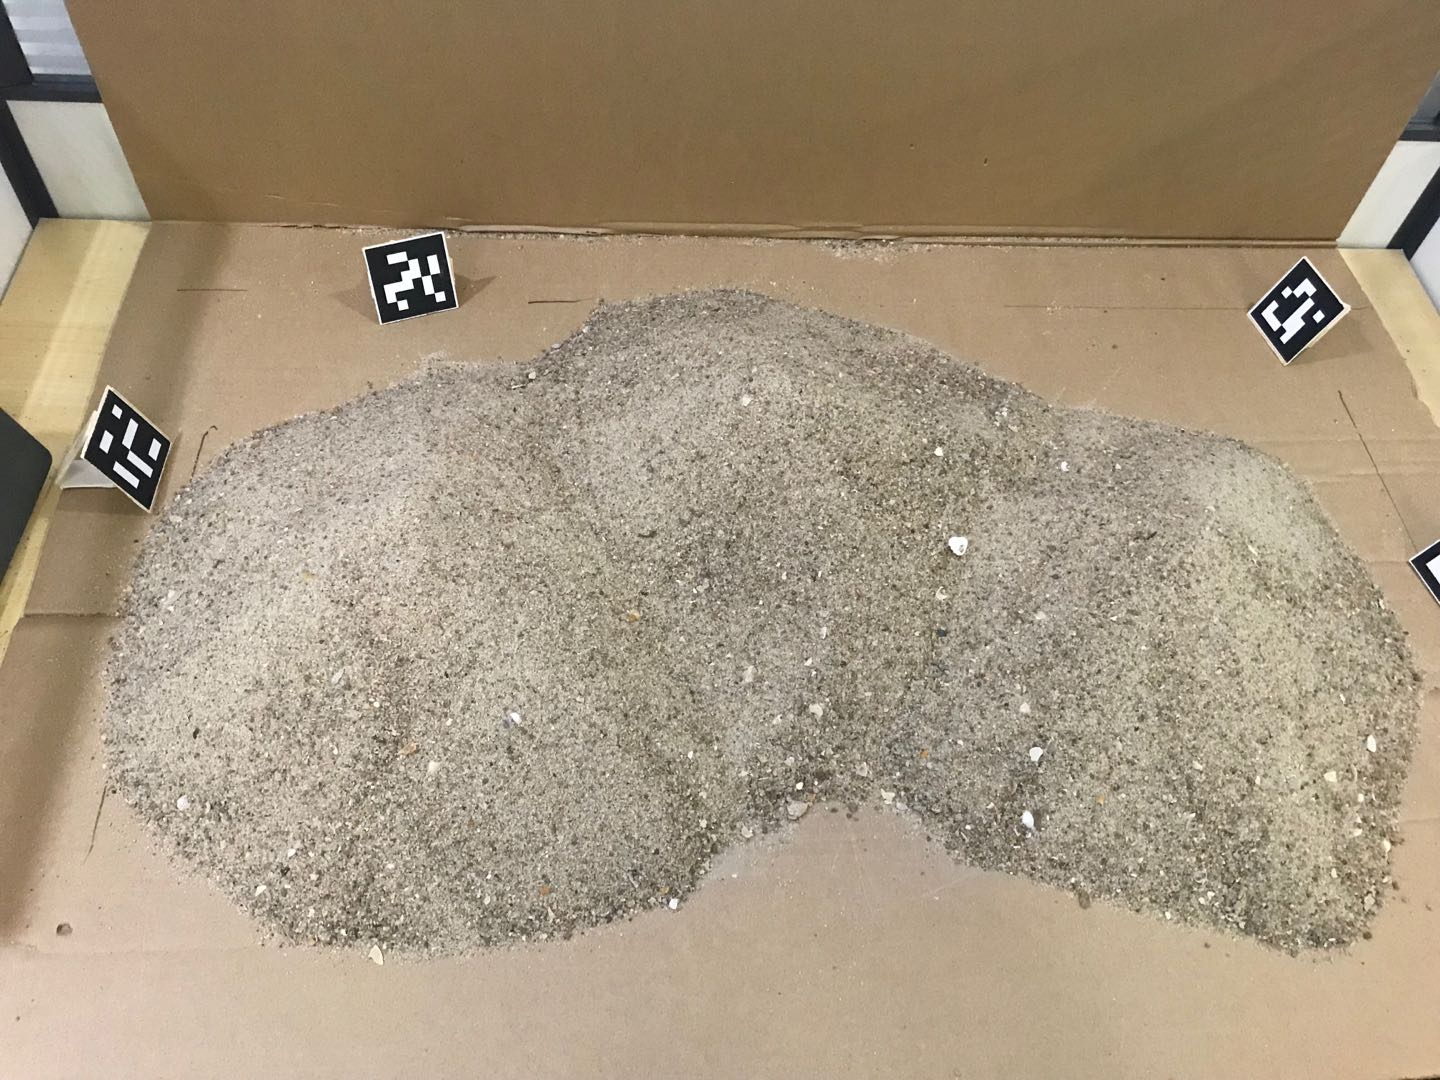
\includegraphics[width=7.5cm, height=5cm]{test_3.png} & 960*455\\
%   \bottomrule
%   \end{tabular}
% \end{table}
% \begin{table}[H]
%   \centering
%   \caption{体积测量结果-\uppercase\expandafter{\romannumeral2}}
%   \label{tab:volume_test_2}
%   \begin{tabular}{C{8cm}C{2.0cm}C{1.2cm}C{3.6cm}}
%   \toprule
%   \textbf{稀疏点云} & \textbf{点集个数} & \textbf{尺度K} & \textbf{误差}\\
%   \midrule
%   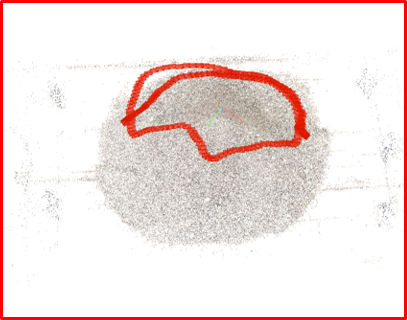
\includegraphics[width=7.5cm, height=5cm]{test_1_sparse.png}  &110149&1.945&-0.0259x-0.0331y-0.0873z+1=0\\
%   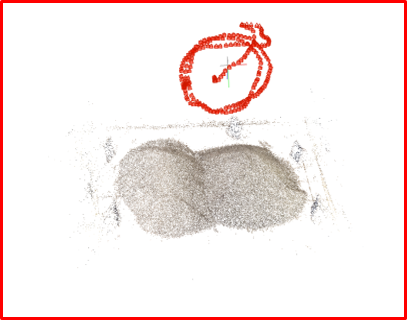
\includegraphics[width=7.5cm, height=5cm]{test_2_sparse.png}  & 86403&8.143& 0.0068x-0.0299y-0.0620z+1=0\\
%   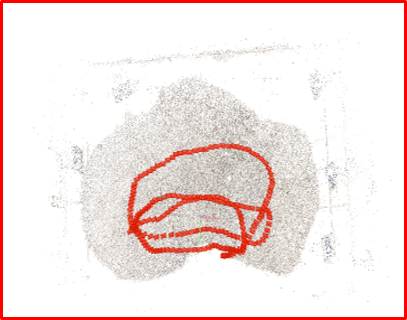
\includegraphics[width=7.5cm, height=5cm]{test_3_sparse.png}  & 83196&3.522& 0.0119x-0.0254y-0.0683z+1=0\\
%   \bottomrule
%   \end{tabular}
% \end{table}
% \begin{table}[t]
%   \centering
%   \caption{体积测量结果-\uppercase\expandafter{\romannumeral3}}
%   \label{tab:volume_test_3}
%   \begin{tabular}{C{8cm}C{2.4cm}C{2.4cm}C{2.0cm}}
%   \toprule
%   \textbf{稠密点云} & \textbf{计算耗时(s)} & \textbf{堆体体积($cm^3$)} & \textbf{测量精度}\\
%   \midrule
%   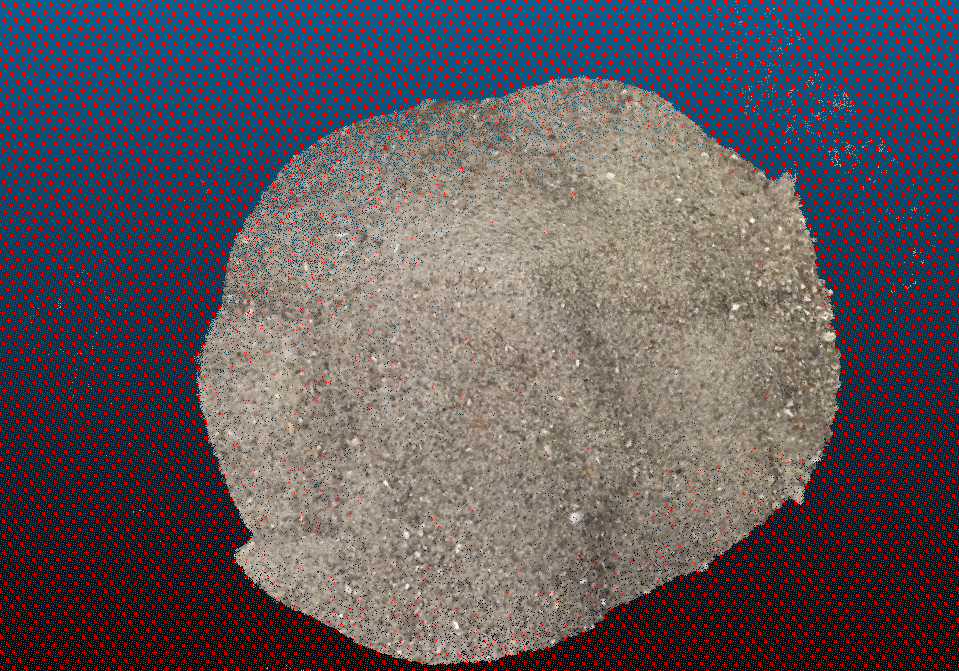
\includegraphics[width=7.5cm, height=5cm]{test_1_dense.png}  & 712 & 10340  &   1.1$\%$\\
%   \includegraphics[width=7.5cm, height=5cm]{test_2_dense.png}  & 675 & 99032  &   0.9$\%$\\
%   \includegraphics[width=7.5cm, height=5cm]{test_3_dense.png}  & 663 & 10552  &   1.3$\%$\\
%   \bottomrule
%   \end{tabular}
% \end{table}

% \begin{figure}[H]
%   \centering
%     \subcaptionbox{单峰堆体场景预览图\label{fig:test_1}}{
%     \includegraphics[height=6cm,width=11.7cm]{test_1.png}}
%   \vskip0.5cm
%     \subcaptionbox{双峰堆体场景预览图\label{fig:test_2}}{
%     \includegraphics[height=6cm,width=11.7cm]{test_2.png}}
%   \vskip0.5cm
%     \subcaptionbox{多峰堆体场景预览图\label{fig:test_3}}{
%     \includegraphics[height=6cm,width=11.7cm]{test_3.png}}
% \caption{不同堆体场景预览图}\label{fig:test}
% \end{figure}

% \begin{figure}[H]
%   \centering
%     \subcaptionbox{单峰堆体场景稀疏点云图\label{fig:test_1_sparse}}{
%     \includegraphics[height=6cm,width=11.7cm]{test_1_sparse.png}}
%   \vskip0.5cm
%     \subcaptionbox{双峰堆体场景稀疏点云图\label{fig:test_2_sparse}}{
%     \includegraphics[height=6cm,width=11.7cm]{test_2_sparse.png}}
%   \vskip0.5cm
%     \subcaptionbox{多峰堆体场景稀疏点云图\label{fig:test_3_sparse}}{
%     \includegraphics[height=6cm,width=11.7cm]{test_3_sparse.png}}
% \caption{不同堆体场景稀疏点云示意图}\label{fig:test_sparse}
% \end{figure}

% \begin{figure}[H]
%   \centering
%     \subcaptionbox{单峰堆体场景稠密点云图\label{fig:test_1_dense}}{
%     \includegraphics[height=6cm,width=11.7cm]{test_1_dense.png}}
%   \vskip0.5cm
%     \subcaptionbox{双峰堆体场景稠密点云图\label{fig:test_2_dense}}{
%     \includegraphics[height=6cm,width=11.7cm]{test_2_dense.png}}
%   \vskip0.5cm
%     \subcaptionbox{多峰堆体场景稠密点云图\label{fig:test_3_dense}}{
%     \includegraphics[height=6cm,width=11.7cm]{test_3_dense.png}}
% \caption{不同堆体场景稠密点云示意图}\label{fig:test_dense}
% \end{figure}

\section{本章小结}
本章分模块测试了无人机在非GPS场景下依靠纯视觉进行定位的效果与精度,以及改进后的三维重建的效果和基于纯视觉的堆体体
积测量算法的准确度和稳定性。

对于无人机的定位系统,高度方向的误差为0.18m,整体误差为0.5m,整体定位精度在5$\%$以内,
对于结合了SLAM结果的三维重建系统,匹配速度和点云模型准确度明显提升,最后的体积测量模块,
可以估计出准确的尺度大小和水平面解析方程,通过对点云体积的求解获得堆体体积,测量误差可以控制在2$\%$以内。
